\chapter{IMPLEMENTASI}
\label{chap:implementasi}

Pada Bab ini dilakukan implementasi dari TOGAF Pertahanan Indonesia yang telah dirancang terhadap konteks nyata Kementerian Pertahanan Republik Indonesia (Kemhan RI). Implementasi dijalankan dengan menelusuri fase dari TOGAF Pertahanan Indonesia secara berurutan, mulai dari fase \textit{Preliminary} hingga fase \textit{Migration Planning}, untuk menghasilkan rancangan arsitektur transformasi digital pertahanan yang aktual bagi Kemhan RI.

\section{Fase \textit{Preliminary}}
\label{sec:impl-preliminary}

Fase \textit{Preliminary} bertujuan untuk membangun fondasi bagi keseluruhan pengembangan arsitektur transformasi digital pertahanan. Fase ini menetapkan prinsip arsitektur yang menjadi pedoman perancangan, ruang lingkup arsitektur yang membatasi objek pengembangan, pemangku kepentingan, struktur tata kelola arsitektur (\textit{architecture governance}), serta repositori arsitektur sebagai wadah penyimpanan artefak. Kelima keluaran tersebut menjadi perangkat kerja yang mengikat seluruh fase berikutnya.

\subsection{Penetapan Prinsip Arsitektur}

Prinsip arsitektur (\textit{architecture principles}) merupakan kaidah fundamental yang mengarahkan seluruh keputusan perancangan agar konsisten antarfase dan antardomain. Prinsip yang digunakan pada implementasi ini adalah kesembilan prinsip arsitektur Pertahanan Indonesia yang telah dirumuskan pada Tabel~\ref{tab:prinsip-arsitektur}. Kesembilan prinsip tersebut dikelompokkan ke dalam enam kategori baku, yaitu prinsip arsitektur umum, prinsip bisnis, prinsip data, prinsip aplikasi, prinsip teknologi, dan prinsip keamanan, sebagaimana diperlihatkan pada Tabel~\ref{tab:pengelompokan-prinsip}.

\begin{longtable}{@{}p{0.30\textwidth}p{0.63\textwidth}@{}}
\caption{Pengelompokan Prinsip Arsitektur Pertahanan ke dalam Enam Kategori}
\label{tab:pengelompokan-prinsip}\\
\toprule
\textbf{Prinsip} & \textbf{Deskripsi}\\
\midrule
\endfirsthead
\multicolumn{2}{c}{\tablename\ \thetable\ (lanjutan)}\\
\toprule
\textbf{Prinsip} & \textbf{Deskripsi}\\
\midrule
\endhead
\bottomrule
\endfoot
\multicolumn{2}{@{}l}{\textbf{A. Prinsip Arsitektur (Umum)}}\\
\addlinespace
\textit{Smart Defence Oriented} & Transformasi digital harus mendukung konsep \textit{smart defence} dan operasi multi-domain.\\
\addlinespace
\textit{Governance \& Compliance} & Seluruh layanan digital harus sesuai dengan regulasi pertahanan, SPBE, dan ketentuan keamanan nasional.\\
\addlinespace
\multicolumn{2}{@{}l}{\textbf{B. Prinsip Bisnis}}\\
\addlinespace
\textit{Integrated Command \& Control} & Mendukung sistem komando dan pengendalian terintegrasi berbasis C5ISR.\\
\addlinespace
\textit{User-Centric Service} & Sistem dibangun untuk meningkatkan efektivitas personel dan kualitas layanan organisasi.\\
\addlinespace
\multicolumn{2}{@{}l}{\textbf{C. Prinsip Data}}\\
\addlinespace
\textit{Data as Strategic Asset} & Data pertahanan diperlakukan sebagai aset strategis nasional untuk mendukung pengambilan keputusan.\\
\addlinespace
\multicolumn{2}{@{}l}{\textbf{D. Prinsip Aplikasi}}\\
\addlinespace
\textit{Interoperabilitas} & Seluruh sistem Kemhan dan ketiga angkatan harus dapat saling terintegrasi dan bertukar data secara \textit{real-time}.\\
\addlinespace
\multicolumn{2}{@{}l}{\textbf{E. Prinsip Teknologi}}\\
\addlinespace
\textit{Scalability \& Flexibility} & Arsitektur harus mampu berkembang mengikuti dinamika ancaman dan kemajuan teknologi di masa depan.\\
\addlinespace
\textit{Availability \& Reliability} & Sistem pertahanan digital harus memiliki ketersediaan tinggi dan tahan terhadap gangguan.\\
\addlinespace
\multicolumn{2}{@{}l}{\textbf{F. Prinsip Keamanan}}\\
\addlinespace
\textit{Security by Design} & Keamanan siber menjadi bagian utama arsitektur sejak tahap perencanaan, bukan sebagai tambahan di akhir.\\
\end{longtable}

\subsection{Penetapan Ruang Lingkup Arsitektur}

Ruang lingkup arsitektur menetapkan batas organisasi, unit, dan domain yang menjadi objek pengembangan. Dari sisi organisasi, ruang lingkup mencakup Kemhan RI sebagai organisasi inti, ketiga matra (TNI Angkatan Darat, Angkatan Laut, dan Angkatan Udara) sebagai entitas yang terhubung melalui interoperabilitas lintas matra, serta industri pertahanan nasional sebagai mitra ekosistem digital.

Dari sisi unit organisasi, penetapan ini mengacu pada struktur terbaru Kemhan berdasarkan Peraturan Menteri Pertahanan Nomor 1 Tahun 2024 tentang Organisasi dan Tata Kerja Kementerian Pertahanan \parencite{Permenhan2024}. Berdasarkan peraturan tersebut, fungsi pengelolaan data dan sistem informasi kini diselenggarakan oleh \textit{Badan Informasi dan Komunikasi Pertahanan}, yang membawahi Pusat Teknologi Informasi dan Komunikasi Pertahanan, Pusat Informasi Strategis Pertahanan, dan Pusat Pertahanan Siber. Unit-unit yang menjadi fokus pengembangan arsitektur meliputi Sekretariat Jenderal, Direktorat Jenderal Potensi Pertahanan, Badan Informasi dan Komunikasi Pertahanan beserta ketiga pusatnya, serta Badan Pengembangan Kebijakan dan Teknologi Pertahanan.

Dari sisi domain arsitektur, dilakukan pengembangan pada lima domain sesuai TOGAF Pertahanan Indonesia, yaitu \textit{Business Architecture}, \textit{Data Architecture}, \textit{Application Architecture}, \textit{Technology Architecture}, dan \textit{C5ISR Architecture}. Sesuai batasan penelitian, ruang lingkup tidak mencakup aspek rahasia militer dan operasi tempur, melainkan difokuskan pada integrasi sistem informasi, keamanan data, dan tata kelola digital pertahanan. Ringkasan ketiga dimensi ruang lingkup dapat dilihat pada Gambar~\ref{fig:ruang-lingkup}.

\begin{figure}[htbp]
\centering
\caption{Ruang Lingkup Arsitektur Transformasi Digital Pertahanan}
\label{fig:ruang-lingkup}
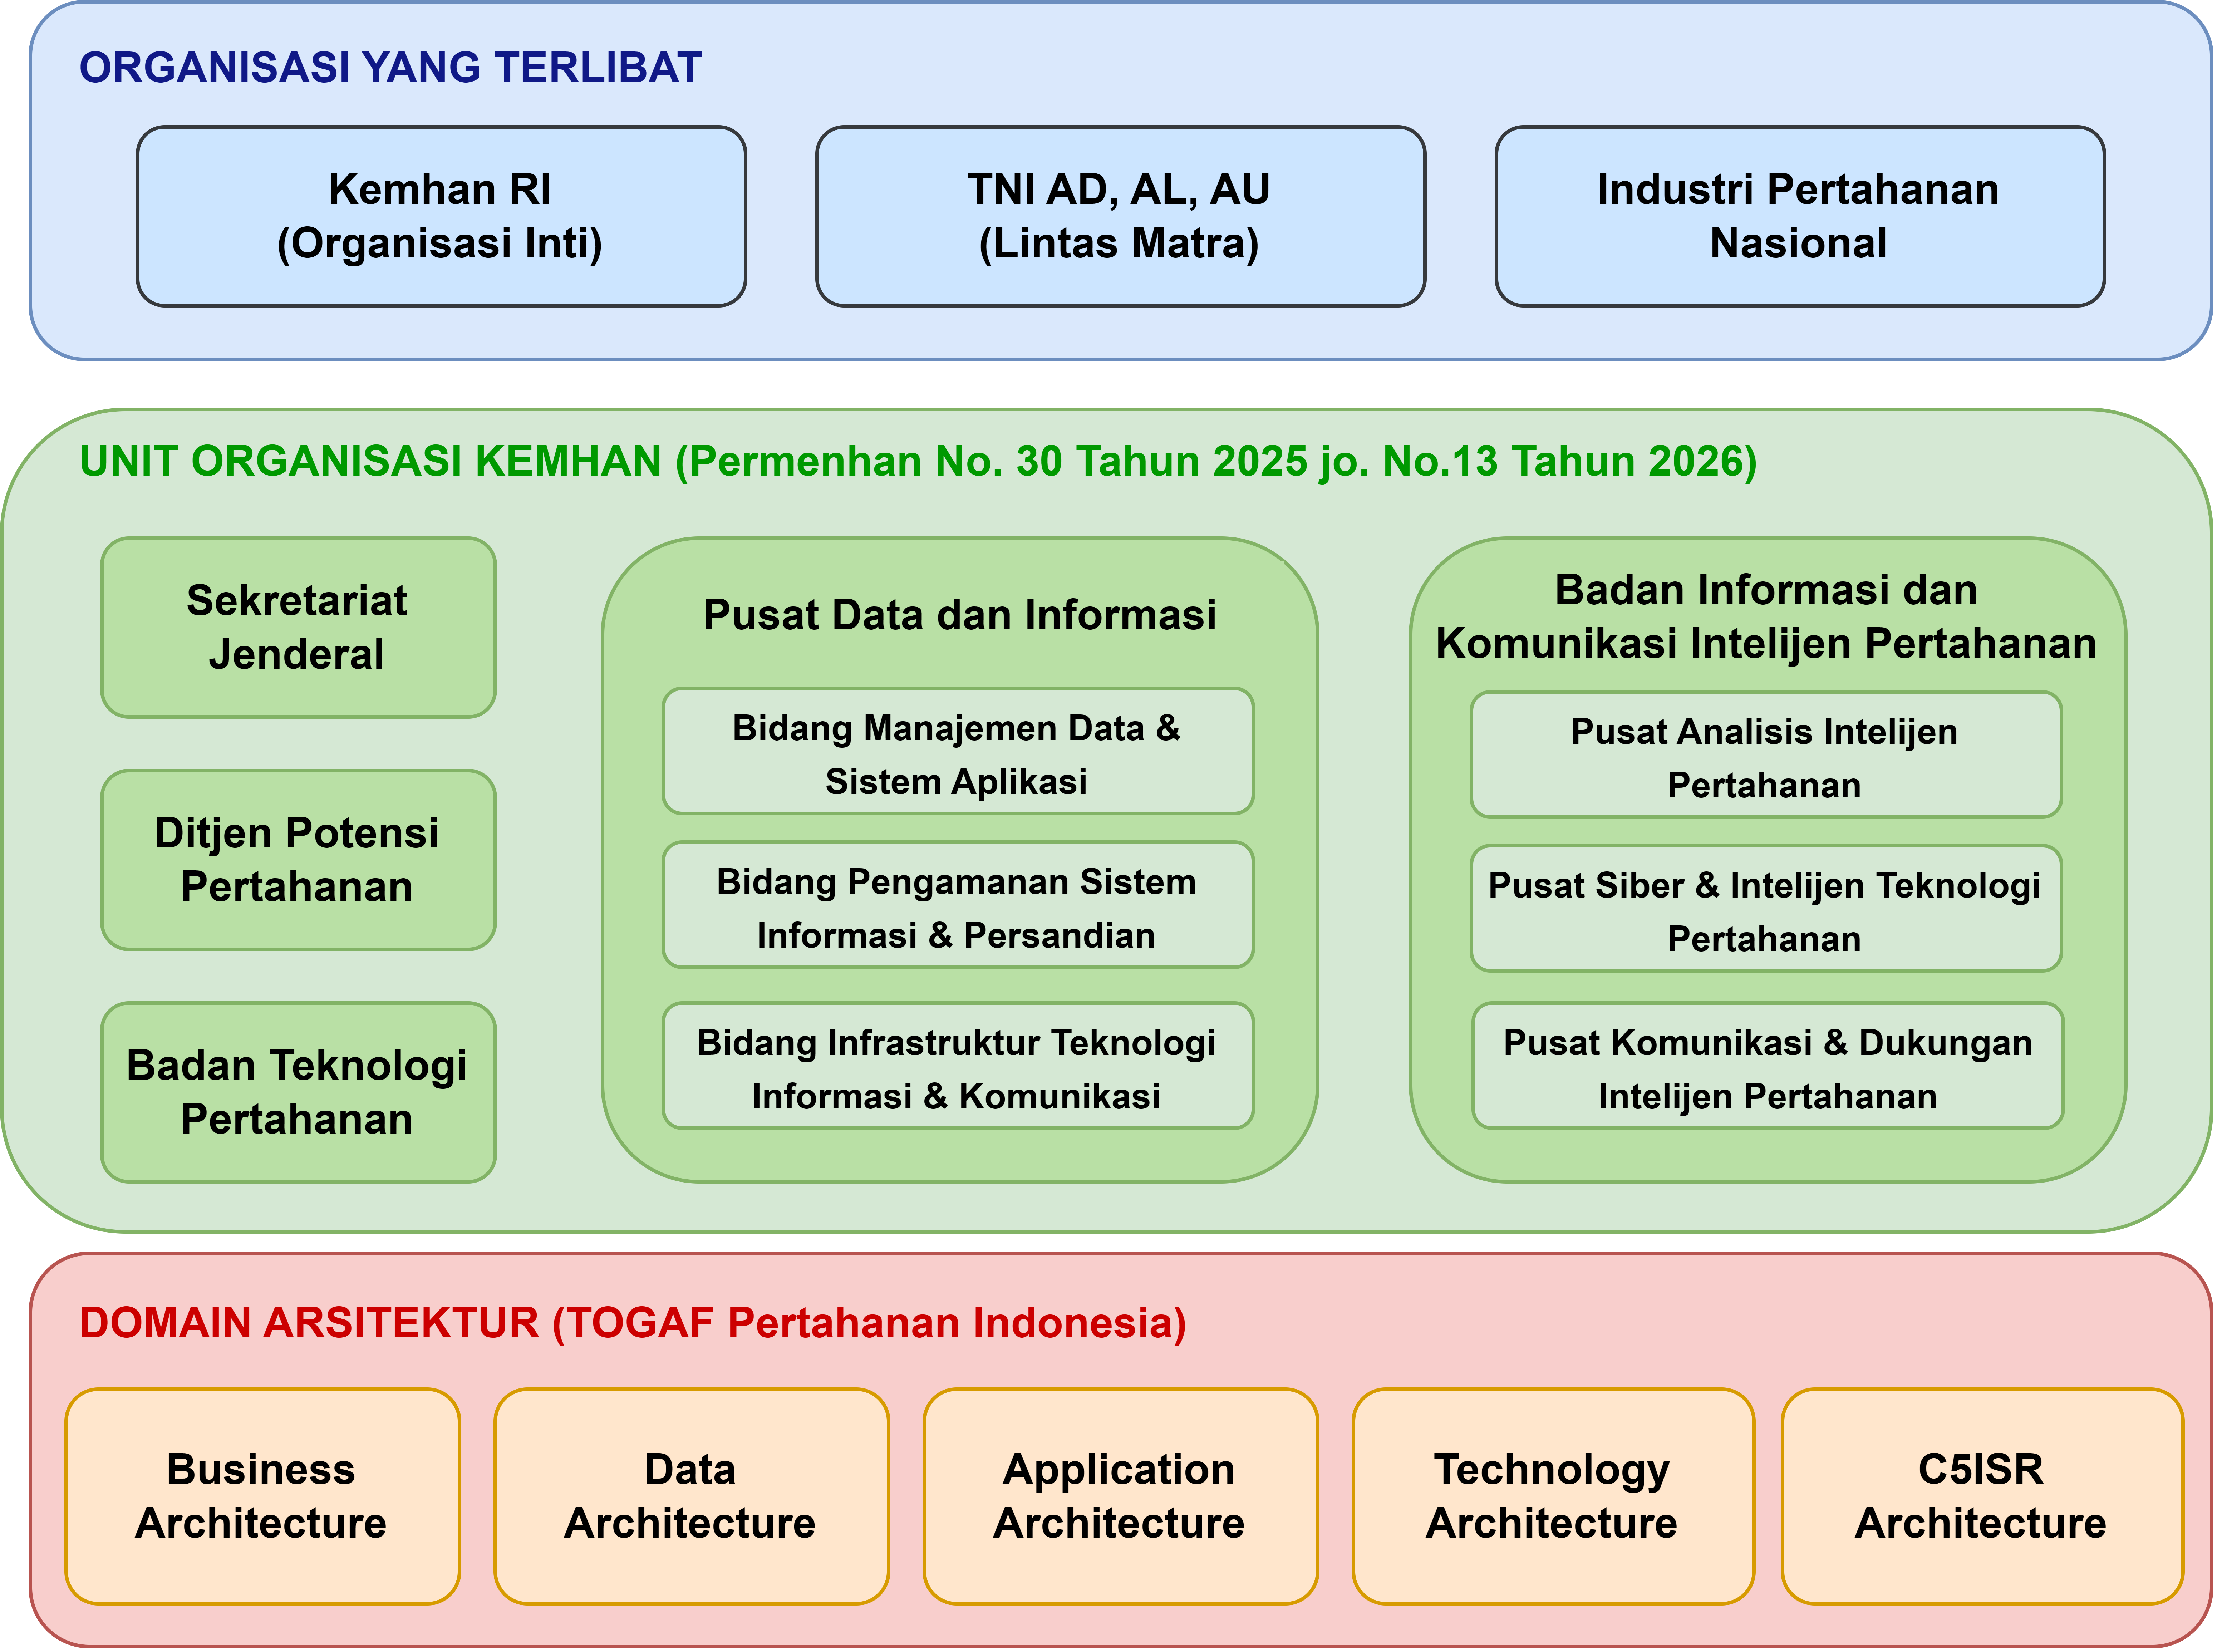
\includegraphics[width=0.85\textwidth]{images/Preliminary - Ruang Lingkup.drawio.png}
\end{figure}

\subsection{Identifikasi \textit{Stakeholder}}

Identifikasi pemangku kepentingan (\textit{stakeholder}) bertujuan mengenali pihak-pihak yang terpengaruh oleh dan atau memengaruhi arsitektur, beserta kepedulian (\textit{concern}), tingkat pengaruh (\textit{influence}), dan kebutuhan utamanya. Pemetaan ini menjadi dasar penyusunan rencana komunikasi dan penentuan prioritas kebutuhan pada fase \textit{Architecture Vision}. Hasil pemetaan disajikan dalam matriks pemangku kepentingan pada Tabel~\ref{tab:stakeholder}.

\begin{longtable}{@{}p{0.04\textwidth}p{0.22\textwidth}p{0.24\textwidth}p{0.13\textwidth}p{0.24\textwidth}@{}}
\caption{Matriks Pemangku Kepentingan (\textit{Stakeholder Matrix})}
\label{tab:stakeholder}\\
\toprule
\textbf{No.} & \textbf{Pemangku Kepentingan} & \textbf{Kepedulian (\textit{Concern})} & \textbf{Pengaruh} & \textbf{Kebutuhan Utama}\\
\midrule
\endfirsthead
\multicolumn{5}{c}{\tablename\ \thetable\ (lanjutan)}\\
\toprule
\textbf{No.} & \textbf{Pemangku Kepentingan} & \textbf{Kepedulian (\textit{Concern})} & \textbf{Pengaruh} & \textbf{Kebutuhan Utama}\\
\midrule
\endhead
\bottomrule
\endfoot
1 & Menteri Pertahanan & Arah strategis dan kedaulatan pertahanan & Sangat Tinggi & Informasi eksekutif dan keputusan berbasis data\\
\addlinespace
2 & Sekretaris Jenderal & Koordinasi dan tata kelola organisasi & Tinggi & Integrasi lintas unit dan kepatuhan SPBE\\
\addlinespace
3 & Kepala Badan Informasi dan Komunikasi Pertahanan & Sistem informasi, komunikasi strategis, dan pertahanan siber & Sangat Tinggi & Infrastruktur TIK terpadu dan keamanan siber\\
\addlinespace
4 & Pusat Pertahanan Siber & Keamanan siber pertahanan & Tinggi & Penerapan \textit{security by design} dan pusat operasi keamanan\\
\addlinespace
5 & Ditjen Potensi Pertahanan & Potensi dan industri pertahanan & Tinggi & Data potensi dan kolaborasi industri pertahanan\\
\addlinespace
6 & Ditjen Strategi dan Perencanaan Pertahanan & Perumusan strategi dan perencanaan & Tinggi & Data perencanaan pertahanan yang terintegrasi\\
\addlinespace
7 & TNI AD, AL, AU & Operasi dan interoperabilitas lintas matra & Tinggi & Pertukaran data dan dukungan komando-kendali\\
\addlinespace
8 & Badan Pengembangan Kebijakan dan Teknologi Pertahanan & Kebijakan dan teknologi pertahanan & Sedang & Standar teknologi dan dukungan inovasi\\
\addlinespace
9 & Industri Pertahanan Nasional & Kolaborasi dan transfer teknologi & Sedang & Standar terbuka dan interoperabilitas\\
\addlinespace
10 & Personel/Pengguna Layanan & Kemudahan dan keandalan layanan & Sedang & Layanan digital yang \textit{user-centric}\\
\end{longtable}

\subsection{Penetapan \textit{Governance}}

Tata kelola arsitektur (\textit{architecture governance}) menetapkan struktur pengambilan keputusan yang menjamin arsitektur dikembangkan dan dipelihara secara terkendali. Meskipun Permenhan Nomor 1 Tahun 2024 telah menaikkan fungsi data, informasi, dan siber ke tingkat Badan, mandat Badan Informasi dan Komunikasi Pertahanan bersifat pengelolaan operasional (\textit{run-the-engine}), sehingga tetap diperlukan fungsi orkestrasi transformasi lintas organisasi yang diperankan oleh \textit{Chief Enterprise Architect} atau \textit{Digital Transformation Officer} (DTO). Struktur tata kelola arsitektur terdiri atas \textit{Architecture Board}, \textit{Architecture Team}, dan pemilik arsitektur (\textit{owner}) sebagaimana diperlihatkan pada Tabel~\ref{tab:governance}.

\begin{longtable}{@{}p{0.04\textwidth}p{0.22\textwidth}p{0.32\textwidth}p{0.32\textwidth}@{}}
\caption{Struktur Tata Kelola Arsitektur (\textit{Architecture Governance})}
\label{tab:governance}\\
\toprule
\textbf{No.} & \textbf{Elemen Tata Kelola} & \textbf{Penanggung Jawab} & \textbf{Peran Utama}\\
\midrule
\endfirsthead
\multicolumn{4}{c}{\tablename\ \thetable\ (lanjutan)}\\
\toprule
\textbf{No.} & \textbf{Elemen Tata Kelola} & \textbf{Penanggung Jawab} & \textbf{Peran Utama}\\
\midrule
\endhead
\bottomrule
\endfoot
1 & \textit{Architecture Board} (Dewan Arsitektur) & Diketuai Sekretaris Jenderal; beranggotakan Kepala Badan Informasi dan Komunikasi Pertahanan, para Direktur Jenderal terkait, dan perwakilan matra & Menetapkan prinsip, menyetujui \textit{Request for Architecture Work}, serta mengesahkan dan meninjau kepatuhan arsitektur\\
\addlinespace
2 & \textit{Architecture Team} (Tim Arsitektur) & Dipimpin \textit{Chief Enterprise Architect} (fungsi DTO), berkedudukan pada Badan Informasi dan Komunikasi Pertahanan & Melaksanakan siklus TOGAF Pertahanan Indonesia dan merancang arsitektur pada domain bisnis, data, aplikasi, teknologi, dan C5ISR\\
\addlinespace
3 & Tim Keamanan Siber & Pusat Pertahanan Siber & Menjamin penerapan prinsip \textit{security by design} pada seluruh fase\\
\addlinespace
4 & Pemilik Arsitektur (\textit{Owner}) & Menteri Pertahanan sebagai pemilik utama; Kepala Badan Informasi dan Komunikasi Pertahanan sebagai pemilik pelaksana & Memiliki, membiayai, dan menjamin keberlanjutan arsitektur transformasi digital pertahanan\\
\end{longtable}

\subsection{Repositori Arsitektur}

Repositori arsitektur (\textit{Architecture Repository}) merupakan wadah penyimpanan seluruh artefak arsitektur agar tertata, konsisten, dan dapat ditelusuri antarfase. Repositori dipartisi menurut domain arsitektur sehingga setiap artefak tersimpan pada bagian yang sesuai. Struktur repositori beserta muatannya dapat dilihat pada Tabel~\ref{tab:repository}.

\begin{longtable}{@{}p{0.30\textwidth}p{0.63\textwidth}@{}}
\caption{Struktur \textit{Repository} Arsitektur}
\label{tab:repository}\\
\toprule
\textbf{Bagian \textit{Repository}} & \textbf{Muatan Utama}\\
\midrule
\endfirsthead
\multicolumn{2}{c}{\tablename\ \thetable\ (lanjutan)}\\
\toprule
\textbf{Bagian \textit{Repository}} & \textbf{Muatan Utama}\\
\midrule
\endhead
\bottomrule
\endfoot
\textit{Business Repository} & Model proses bisnis, peta kapabilitas, \textit{value stream}, dan struktur organisasi pertahanan\\
\addlinespace
\textit{Data Repository} & Model dan kamus data, katalog serta metadata, dan standar Satu Data Pertahanan\\
\addlinespace
\textit{Application Repository} & Portofolio dan katalog aplikasi pertahanan beserta keterkaitannya\\
\addlinespace
\textit{Technology Repository} & Standar teknologi, katalog infrastruktur, platform, dan protokol keamanan\\
\addlinespace
\textit{C5ISR Repository} & Model arsitektur C5ISR (komando-kendali, komunikasi, komputer, siber, intelijen, surveilans, dan pengintaian), rantai \textit{sensor-to-shooter}, dan \textit{common operational picture} berbasis \textit{network centric warfare}\\
\addlinespace
\textit{Reference Library} dan Standar & Prinsip arsitektur, katalog regulasi (SPBE, Satu Data), dan model rujukan TOGAF Pertahanan Indonesia\\
\end{longtable}

\section{Fase \textit{Architecture Vision}}
\label{sec:impl-vision}

Fase \textit{Architecture Vision} merumuskan visi, misi, dan tujuan strategis arsitektur transformasi digital pertahanan, serta memberikan gambaran tingkat tinggi mengenai kondisi target (\textit{to-be}) yang ingin dicapai. Fase ini menerima masukan dari keluaran fase \textit{Preliminary} ditambah kerangka regulasi nasional serta doktrin dan strategi pertahanan dan menghasilkan Dokumen \textit{Architecture Vision}, tujuan strategis, penilaian kapabilitas dan kesiapan, proposisi nilai dan \textit{Statement of Architecture Work} yang menjadi acuan bagi seluruh fase pengembangan domain.

\subsection{Visi, Misi dan Tujuan Arsitektur}

Visi arsitektur menetapkan arah jangka panjang transformasi digital pertahanan Kemhan RI yang dirumuskan sebagai berikut.

\begin{quote}
\itshape\bfseries ``Terwujudnya arsitektur transformasi digital pertahanan yang terintegrasi, aman, dan berorientasi smart defence untuk mewujudkan keunggulan informasi serta mendukung pengambilan keputusan yang cepat dan tepat di lingkungan Kemhan RI dan TNI.''
\end{quote}

Untuk mewujudkan visi tersebut, ditetapkan misi arsitektur sebagai berikut:
\begin{enumerate}
\item Mewujudkan interoperabilitas dan integrasi data lintas unit Kemhan dan ketiga matra;
\item Menerapkan keamanan siber sejak perancangan (\textit{security by design}) pada seluruh sistem pertahanan;
\item Menyediakan layanan digital yang andal dan berorientasi pengguna bagi personel dan pimpinan;
\item Membangun fondasi kapabilitas C5ISR untuk mendukung komando dan kendali terintegrasi; dan
\item Menyelenggarakan tata kelola digital yang selaras dengan SPBE dan Satu Data Indonesia.
\end{enumerate}

Visi dan misi tersebut diturunkan menjadi tujuan strategis arsitektur yang masing-masing tertaut pada prinsip arsitektur pertahanan, sebagaimana disajikan pada Tabel~\ref{tab:tujuan-strategis}.

\begin{longtable}{@{}p{0.04\textwidth}p{0.58\textwidth}p{0.31\textwidth}@{}}
\caption{Tujuan Strategis Arsitektur dan Keterkaitan Prinsip}
\label{tab:tujuan-strategis}\\
\toprule
\textbf{No.} & \textbf{Tujuan Strategis} & \textbf{Keterkaitan Prinsip}\\
\midrule
\endfirsthead
\multicolumn{3}{c}{\tablename\ \thetable\ (lanjutan)}\\
\toprule
\textbf{No.} & \textbf{Tujuan Strategis} & \textbf{Keterkaitan Prinsip}\\
\midrule
\endhead
\bottomrule
\endfoot
1 & Mewujudkan integrasi data dan sistem lintas Kemhan dan matra & \textit{Interoperabilitas}\\
\addlinespace
2 & Memperkuat keamanan siber pertahanan secara menyeluruh & \textit{Security by Design}\\
\addlinespace
3 & Mengelola data pertahanan sebagai aset strategis pengambilan keputusan & \textit{Data as Strategic Asset}\\
\addlinespace
4 & Menyiapkan kapabilitas C5ISR dan komando-kendali terintegrasi & \textit{Integrated Command \& Control}\\
\addlinespace
5 & Meningkatkan kualitas layanan dan efektivitas personel & \textit{User-Centric Service}\\
\addlinespace
6 & Menjamin kepatuhan tata kelola digital pertahanan & \textit{Governance \& Compliance}\\
\end{longtable}

\subsection{Pendorong dan Kendala Transformasi}

Perumusan visi dilengkapi dengan konfirmasi pendorong (\textit{drivers}) yang mendasari transformasi serta kendala (\textit{constraints}) yang membatasi ruang geraknya. Keduanya menjadi konteks yang memastikan arsitektur target realistis dan selaras dengan arah kebijakan pertahanan nasional, sebagaimana dirangkum pada Tabel~\ref{tab:pendorong-kendala}.

\begin{longtable}{@{}p{0.24\textwidth}p{0.69\textwidth}@{}}
\caption{Pendorong dan Kendala Transformasi Digital Pertahanan}
\label{tab:pendorong-kendala}\\
\toprule
\textbf{Aspek} & \textbf{Uraian}\\
\midrule
\endfirsthead
\multicolumn{2}{c}{\tablename\ \thetable\ (lanjutan)}\\
\toprule
\textbf{Aspek} & \textbf{Uraian}\\
\midrule
\endhead
\bottomrule
\endfoot
Pendorong (\textit{Drivers}) & Arah modernisasi pertahanan pada RPJPN 2025--2045; kebijakan SPBE dan Satu Data Indonesia; meningkatnya ancaman siber dan tuntutan operasi multi-domain; kebutuhan interoperabilitas lintas matra; serta tuntutan pengambilan keputusan berbasis data.\\
\addlinespace
Kendala (\textit{Constraints}) & Fragmentasi sistem dan data silo pada kondisi saat ini; keterbatasan sumber daya manusia digital; keberadaan sistem lama (\textit{legacy}); aspek kerahasiaan dan keamanan pertahanan; serta keterbatasan anggaran dan waktu.\\
\end{longtable}

\subsection{Penilaian Kapabilitas dan Kesiapan Transformasi}

Penilaian kapabilitas (\textit{capability assessment}) dan kesiapan transformasi bertujuan mengukur sejauh mana organisasi mampu menjalankan perubahan yang diusung arsitektur target. Penilaian dilakukan terhadap faktor kepemimpinan, sumber daya manusia, data, infrastruktur, keamanan, serta regulasi, dengan hasil disajikan pada Tabel~\ref{tab:kesiapan}.

\begin{longtable}{@{}p{0.04\textwidth}p{0.24\textwidth}p{0.44\textwidth}p{0.19\textwidth}@{}}
\caption{Penilaian Kesiapan Transformasi (\textit{Readiness Assessment})}
\label{tab:kesiapan}\\
\toprule
\textbf{No.} & \textbf{Faktor Kesiapan} & \textbf{Kondisi Saat Ini} & \textbf{Tingkat Kesiapan}\\
\midrule
\endfirsthead
\multicolumn{4}{c}{\tablename\ \thetable\ (lanjutan)}\\
\toprule
\textbf{No.} & \textbf{Faktor Kesiapan} & \textbf{Kondisi Saat Ini} & \textbf{Tingkat Kesiapan}\\
\midrule
\endhead
\bottomrule
\endfoot
1 & Kepemimpinan dan tata kelola & Fungsi data dan siber telah menjadi Badan, namun mandat transformasi belum terpusat (Permenhan No. 1 Tahun 2024) & Sedang\\
\addlinespace
2 & Sumber daya manusia digital & Kompetensi digital masih terbatas dan tersebar antarunit & Rendah--Sedang\\
\addlinespace
3 & Data dan interoperabilitas & Data masih tersilo dan standar antarunit belum seragam & Rendah\\
\addlinespace
4 & Infrastruktur teknologi & Infrastruktur tersedia tetapi belum sepenuhnya terpadu & Sedang\\
\addlinespace
5 & Keamanan siber & Telah terbentuk Pusat Pertahanan Siber sebagai fondasi & Sedang\\
\addlinespace
6 & Regulasi dan kebijakan & Dukungan SPBE, Satu Data, dan RPJPN 2025--2045 & Tinggi\\
\end{longtable}

\subsection{Identifikasi Risiko dan Mitigasi}

Identifikasi risiko transformasi dilakukan untuk mengantisipasi hambatan yang dapat menggagalkan pencapaian arsitektur target, disertai tindakan mitigasi bagi setiap risiko. Ringkasannya disajikan pada Tabel~\ref{tab:risiko}.

\begin{longtable}{@{}p{0.04\textwidth}p{0.26\textwidth}p{0.26\textwidth}p{0.34\textwidth}@{}}
\caption{Risiko Transformasi dan Mitigasi}
\label{tab:risiko}\\
\toprule
\textbf{No.} & \textbf{Risiko} & \textbf{Dampak} & \textbf{Mitigasi}\\
\midrule
\endfirsthead
\multicolumn{4}{c}{\tablename\ \thetable\ (lanjutan)}\\
\toprule
\textbf{No.} & \textbf{Risiko} & \textbf{Dampak} & \textbf{Mitigasi}\\
\midrule
\endhead
\bottomrule
\endfoot
1 & Resistensi perubahan organisasi & Adopsi arsitektur berjalan lambat & Manajemen perubahan, dukungan pimpinan, dan fungsi DTO\\
\addlinespace
2 & Keterbatasan SDM digital & Kualitas implementasi menurun & Pelatihan, rekrutmen, dan kerja sama kelembagaan\\
\addlinespace
3 & Kompleksitas integrasi sistem \textit{legacy} & Keterlambatan dan pembengkakan biaya & Pentahapan, penggunaan \textit{middleware}/API, dan standar terbuka\\
\addlinespace
4 & Ancaman siber selama transisi & Kebocoran atau gangguan data & Penerapan \textit{security by design} dan penguatan Pusat Pertahanan Siber\\
\addlinespace
5 & Ketergantungan pada teknologi asing & Risiko terhadap kedaulatan data & Mengutamakan teknologi dalam negeri dan standar terbuka\\
\addlinespace
6 & Keterbatasan anggaran dan waktu & Cakupan target tidak tercapai & Prioritas berbasis nilai dan peta jalan bertahap\\
\end{longtable}

\subsection{Konsep Solusi}

Konsep solusi memberikan gambaran menyeluruh mengenai kondisi target arsitektur transformasi digital pertahanan. Konsep ini disusun berlapis, mulai dari infrastruktur terpadu sebagai fondasi, platform interoperabilitas dan Satu Data Pertahanan sebagai simpul integrasi, kapabilitas C5ISR sebagai inti operasional, hingga layanan digital yang melayani seluruh pemangku kepentingan. Keamanan siber berlapis (\textit{security by design}) serta tata kelola \& kepatuhan terhadap SPBE, Satu Data Indonesia, dan regulasi pertahanan membentang menyilang pada seluruh lapisan. Gambaran konsep solusi disajikan pada Gambar~\ref{fig:konsep-solusi}.

\begin{figure}[htbp]
\centering
\caption{Konsep Solusi Arsitektur Target Transformasi Digital Pertahanan}
\label{fig:konsep-solusi}
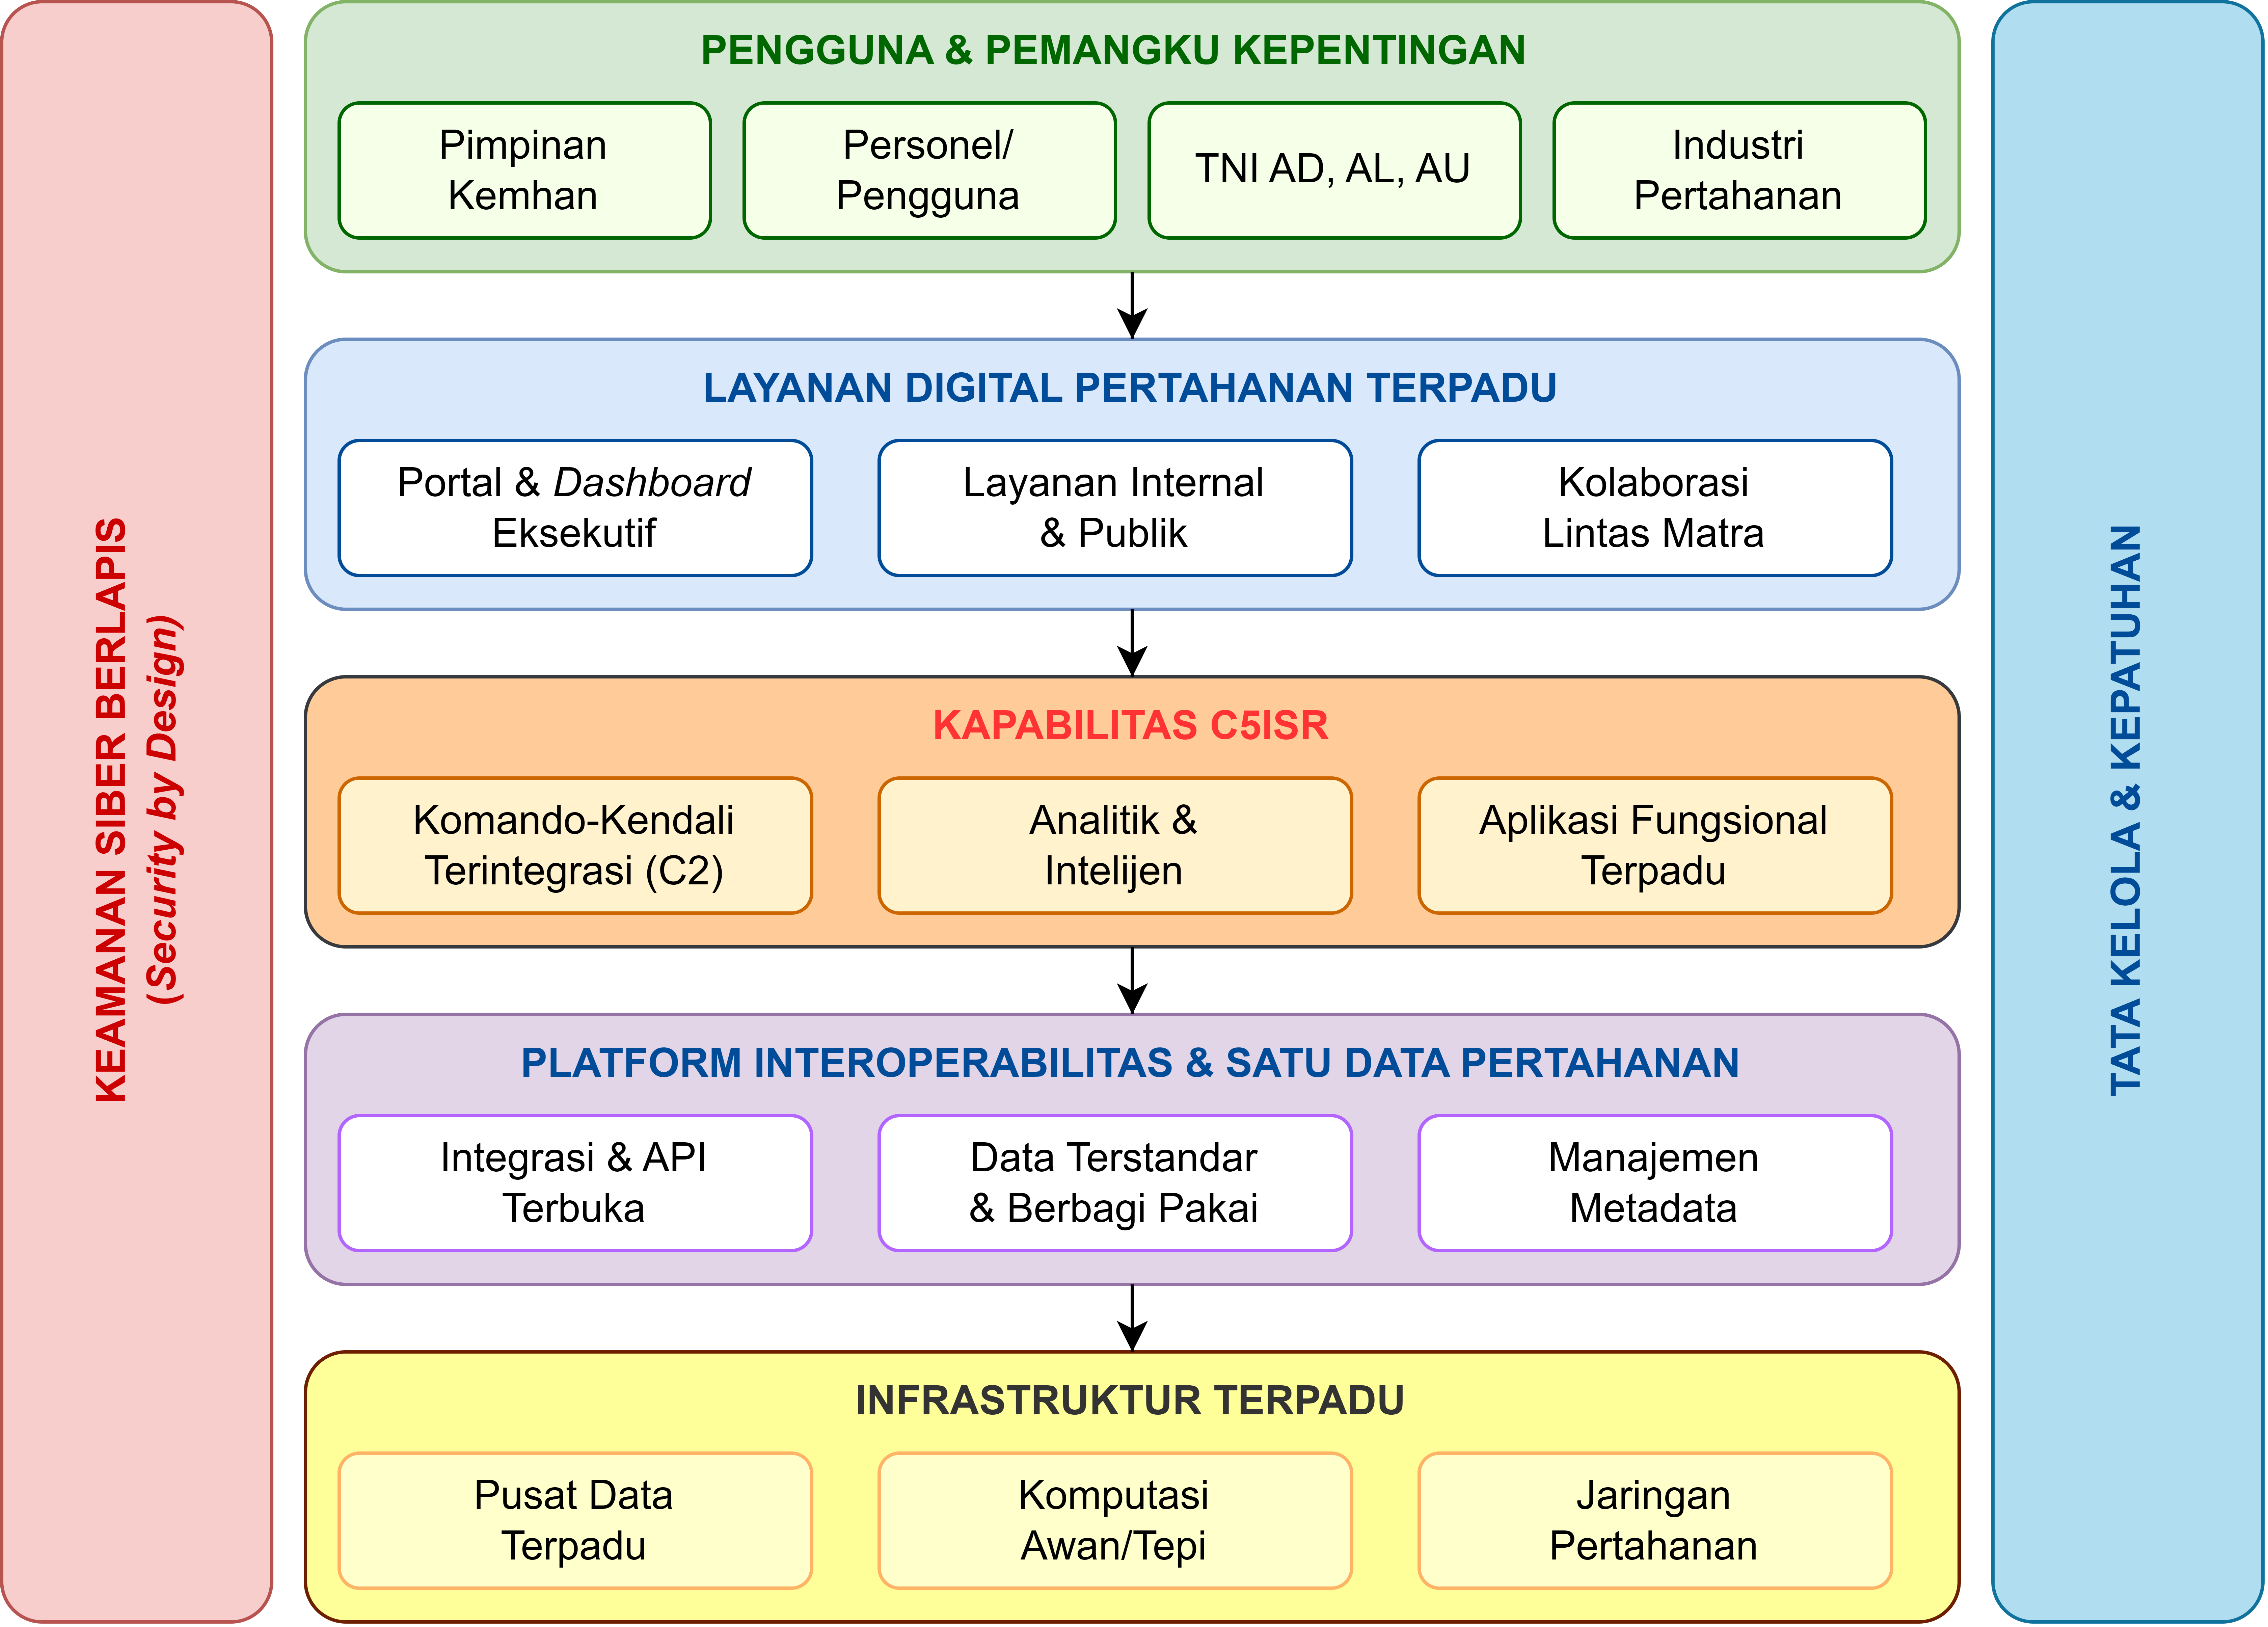
\includegraphics[width=0.85\textwidth]{images/Solusi Arsitektur Target.drawio.png}
\end{figure}

\subsection{\textit{Statement of Architecture Work}}

\textit{Statement of Architecture Work} (SoAW) merupakan dokumen kesepakatan kerja yang menetapkan ruang lingkup, tujuan, keluaran, pelaksana, dan batasan pekerjaan arsitektur untuk memperoleh persetujuan resmi. Ringkasan SoAW disajikan pada Tabel~\ref{tab:soaw}.

\begin{longtable}{@{}p{0.28\textwidth}p{0.65\textwidth}@{}}
\caption{Ringkasan \textit{Statement of Architecture Work}}
\label{tab:soaw}\\
\toprule
\textbf{Komponen} & \textbf{Uraian}\\
\midrule
\endfirsthead
\multicolumn{2}{c}{\tablename\ \thetable\ (lanjutan)}\\
\toprule
\textbf{Komponen} & \textbf{Uraian}\\
\midrule
\endhead
\bottomrule
\endfoot
Nama Pekerjaan & Perancangan arsitektur transformasi digital pertahanan cerdas Kemhan RI berbasis TOGAF Pertahanan Indonesia\\
\addlinespace
Ruang Lingkup & Kemhan RI, ketiga matra, dan industri pertahanan; lima domain arsitektur (bisnis, data, aplikasi, teknologi, dan C5ISR); mengecualikan rahasia militer dan operasi tempur\\
\addlinespace
Tujuan & Mewujudkan arsitektur yang terintegrasi, aman, dan berorientasi \textit{smart defence} sesuai visi dan tujuan strategis\\
\addlinespace
Keluaran (\textit{Deliverables}) & Arsitektur \textit{baseline} dan target tiap domain, peta jalan migrasi, serta instrumen evaluasi arsitektur\\
\addlinespace
Organisasi Pelaksana & \textit{Architecture Board}, \textit{Architecture Team} (fungsi DTO/\textit{Chief Enterprise Architect}), dan Tim Keamanan Siber\\
\addlinespace
Prinsip dan Batasan & Kesembilan prinsip arsitektur (Tabel~\ref{tab:pengelompokan-prinsip}) serta kepatuhan terhadap SPBE, Satu Data Indonesia, dan regulasi pertahanan\\
\addlinespace
Jadwal & Dilaksanakan bertahap mengikuti siklus TOGAF Pertahanan Indonesia dari fase \textit{Preliminary} hingga \textit{Migration Planning}\\
\end{longtable}

\section{Fase \textit{Business Architecture}}
\label{sec:impl-business}

Fase \textit{Business Architecture} bertujuan untuk memperjelas visi arsitektur yang telah dirumuskan pada fase \textit{Architecture Vision} menjadi rancangan proses bisnis, kapabilitas, dan struktur organisasi pertahanan. Fase ini bertitik tolak dari kondisi organisasi Kemhan RI saat ini (\textit{baseline}), kemudian menyusun aliran nilai (\textit{value stream}) dan peta kapabilitas sebagai representasi fungsi pertahanan yang bebas dari sekat unit, untuk selanjutnya merumuskan arsitektur bisnis target (\textit{to-be}) beserta analisis kesenjangannya. Seluruh rancangan mengacu pada struktur organisasi dan tata kerja Kemhan RI sebagaimana ditetapkan dalam Peraturan Menteri Pertahanan Nomor 1 Tahun 2024 tentang Organisasi dan Tata Kerja Kementerian Pertahanan \parencite{Permenhan2024}.

\subsection{Struktur Organisasi dan Tata Kelola}

Arsitektur bisnis \textit{baseline} menggambarkan struktur organisasi dan tata kelola Kemhan RI yang berjalan pada kondisi saat ini. Pemahaman dari struktur ini penting sebagai dasar untuk mengidentifikasi fungsi yang telah ada maupun fungsi yang belum memiliki penanggung jawab. Struktur organisasi Kemhan RI berdasarkan Permenhan Nomor 1 Tahun 2024 disajikan pada Gambar~\ref{fig:struktur-baseline}.

\begin{figure}[htbp]
\centering
\caption{Struktur Organisasi dan Tata Kerja Kemhan RI}
\label{fig:struktur-baseline}
\includegraphics[width=0.9\textwidth]{images/Struktur Organisasi Kemhan Permenhan 30_2025 dan 13_2026.drawio.png}
\end{figure}

Berdasarkan Gambar~\ref{fig:struktur-baseline}, Kemhan RI dipimpin oleh Menteri Pertahanan yang dibantu oleh Wakil Menteri Pertahanan. Di bawahnya terdapat unsur pembantu pimpinan dan pelaksana, yaitu Sekretariat Jenderal, Inspektorat Jenderal, dan empat direktorat jenderal (Strategi Pertahanan, Perencanaan Pertahanan, Potensi Pertahanan, serta Kekuatan Pertahanan), yang dilengkapi unsur pendukung berupa sejumlah badan dan pusat. Fungsi dari pengelolaan data, sistem informasi, komunikasi strategis, dan pertahanan siber diselenggarakan oleh Badan Informasi dan Komunikasi Pertahanan yang membawahi Pusat Teknologi Informasi dan Komunikasi Pertahanan, Pusat Informasi Strategis Pertahanan, dan Pusat Pertahanan Siber. Fungsi utama unit organisasi Kemhan RI dirangkum pada Tabel~\ref{tab:fungsi-unit}.

\begin{longtable}{@{}p{0.04\textwidth}p{0.30\textwidth}p{0.59\textwidth}@{}}
\caption{Fungsi Utama Unit Organisasi Kemhan RI}
\label{tab:fungsi-unit}\\
\toprule
\textbf{No.} & \textbf{Unit Organisasi} & \textbf{Fungsi Utama}\\
\midrule
\endfirsthead
\multicolumn{3}{c}{\tablename\ \thetable\ (lanjutan)}\\
\toprule
\textbf{No.} & \textbf{Unit Organisasi} & \textbf{Fungsi Utama}\\
\midrule
\endhead
\bottomrule
\endfoot
1 & Inspektorat Jenderal & Penyelenggaraan pengawasan keuangan intern di lingkungan Kemhan\\
\addlinespace
2 & Sekretariat Jenderal & Koordinasi pelaksanaan tugas, pembinaan, dan dukungan administrasi seluruh unsur Kemhan\\
\addlinespace
3 & Staf Ahli & Pemberian rekomendasi atas isu-isu strategis kepada Menteri sesuai bidang masing-masing\\
\addlinespace
4 & Ditjen Strategi Pertahanan & Perumusan dan pelaksanaan kebijakan di bidang strategi pertahanan\\
\addlinespace
5 & Ditjen Perencanaan Pertahanan & Perumusan dan pelaksanaan kebijakan di bidang perencanaan pertahanan\\
\addlinespace
6 & Ditjen Potensi Pertahanan & Perumusan dan pelaksanaan kebijakan di bidang potensi pertahanan, termasuk pembinaan industri pertahanan\\
\addlinespace
7 & Ditjen Kekuatan Pertahanan & Perumusan dan pelaksanaan kebijakan di bidang kekuatan pertahanan\\
\addlinespace
8 & Badan Sarana Pertahanan & Pengelolaan sarana pertahanan\\
\addlinespace
9 & Badan Pengembangan Kebijakan dan Teknologi Pertahanan & Pengembangan kebijakan dan teknologi di bidang pertahanan\\
\addlinespace
10 & Badan Pendidikan dan Pelatihan & Penyelenggaraan pendidikan dan pelatihan di bidang pertahanan\\
\addlinespace
11 & Badan Informasi dan Komunikasi Pertahanan & Pengelolaan sistem informasi dan komunikasi strategis pertahanan serta pertahanan siber\\
\addlinespace
12 & Pusat Kelaikan & Dukungan substantif di bidang sertifikasi kelaikan alat peralatan pertahanan dan keamanan, konstruksi pertahanan, satwa pertahanan, serta jaminan mutu fasilitas pertahanan\\
\addlinespace
13 & Pusat Rehabilitasi & Dukungan substantif di bidang rehabilitasi medik, vokasional, sosial, dan perumahsakitan\\
\addlinespace
14 & Pusat Pelaporan dan Pembinaan Keuangan Pertahanan & Penyelenggaraan pelaporan keuangan dan pembinaan pengelolaan keuangan pertahanan\\
\addlinespace
15 & Pusat Pengelolaan Kawasan & Pengelolaan pengamanan, pemeliharaan bangunan, serta pengembangan kerja sama dan instalasi di Kawasan IPSC\\
\end{longtable}

Dari sisi tata kelola, pengambilan keputusan pertahanan berjalan berjenjang dari Menteri Pertahanan ke unit-unit eselon I dengan Sekretariat Jenderal sebagai koordinator lintas unit. Meskipun demikian, pengelolaan teknologi informasi dan data pada kondisi \textit{baseline} sebagian besar masih bersifat operasional pada masing-masing unit, sehingga proses bisnis dijalankan dengan sistem yang terfragmentasi dan data yang tersilo antarunit. Kondisi ini menunjukkan bahwa struktur saat ini belum memiliki unit yang secara khusus memegang mandat transformasi digital lintas organisasi.

\subsection{\textit{Value Stream} Kemhan RI}

\textit{Value stream} Kemhan RI menggambarkan rangkaian aliran nilai yang menghasilkan luaran pertahanan bagi negara, mulai dari perumusan strategi pertahanan hingga pengelolaan SDM dan aset pertahanan. \textit{Value stream} dibuat untuk melihat penyelenggaraan pertahanan sebagai aliran horizontal lintas unit, sehingga membantu mengidentifikasi kapabilitas yang benar-benar ada tanpa terikat pada sekat organisasi. \textit{Value stream} Kemhan RI disajikan pada Gambar~\ref{fig:value-stream}.

\begin{figure}[htbp]
\centering
\caption{\textit{Value Stream} Kemhan RI}
\label{fig:value-stream}
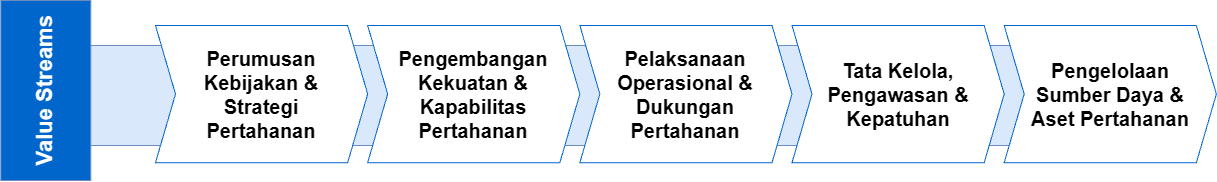
\includegraphics[width=0.9\textwidth]{images/Value Stream Kemhan.drawio.png}
\end{figure}

Gambar~\ref{fig:value-stream} memperlihatkan lima aliran nilai utama yang saling berurutan. Aliran pertama, Perumusan Kebijakan dan Strategi Pertahanan, berfokus untuk menetapkan arah strategis pertahanan nasional yang selaras dengan kepentingan negara dan dinamika global, mencakup penyusunan kebijakan serta perencanaan pertahanan jangka pendek, menengah, dan panjang. Aliran kedua, Pengembangan Kekuatan dan Kapabilitas Pertahanan, berfokus untuk membangun kemampuan pertahanan melalui sumber daya manusia, alutsista, dan infrastruktur strategis. Aliran ketiga, Pelaksanaan Operasional dan Dukungan Pertahanan, berfokus menjalankan kegiatan pertahanan secara efektif dan terkoordinasi dari pusat hingga daerah. Aliran keempat, Tata Kelola, Pengawasan, dan Kepatuhan, berfokus untuk menjamin akuntabilitas, transparansi, serta kepatuhan terhadap regulasi dan standar. Aliran kelima, Pengelolaan Sumber Daya dan Aset Pertahanan, berfokus untuk mengoptimalkan penggunaan sumber daya dan aset negara, termasuk pengelolaan barang milik negara dan keuangan pertahanan. Kelima aliran nilai ini menjadi dasar penurunan kapabilitas yang diperlukan pada peta kapabilitas pertahanan.

\subsection{Peta Kapabilitas Kemhan RI}

Peta kapabilitas Kemhan RI (\textit{business capability map}) menjabarkan kemampuan yang harus dimiliki organisasi untuk menjalankan kelima aliran nilai, terlepas dari unit yang melaksanakannya. Pendekatan yang digunakan berbasis kapabilitas untuk memisahkan ``apa yang dilakukan'' dari ``siapa yang melakukannya'', sehingga arsitektur tetap stabil meskipun terjadi penataan organisasi. Peta kapabilitas Kemhan RI disajikan pada Gambar~\ref{fig:kapabilitas-baseline}.

\begin{figure}[htbp]
\centering
\caption{Peta Kapabilitas Kemhan RI (\textit{Baseline})}
\label{fig:kapabilitas-baseline}
\includegraphics[width=0.75\textwidth]{images/Value Stream & Business Capability Map Kemhan.drawio.png}
\end{figure}

Gambar~\ref{fig:kapabilitas-baseline} menyusun kapabilitas ke dalam tiga lapis. Lapis \textit{defining} memuat kapabilitas utama yang selaras dengan kelima aliran nilai, mulai dari analisis lingkungan strategis dan perumusan kebijakan, pengelolaan alutsista dan pengembangan sumber daya manusia, pelaksanaan operasi serta manajemen komando dan koordinasi, manajemen tata kelola dan pengawasan, hingga manajemen aset, keuangan, dan logistik. Lapis \textit{shared} memuat kapabilitas bersama yang digunakan lintas fungsi, yaitu manajemen sumber daya manusia, manajemen data dan informasi yang mencakup tata kelola data, kualitas data, serta integrasi dan interoperabilitas, selanjutnya ada manajemen hubungan serta komunikasi organisasi. Lapis \textit{enabling} memuat kapabilitas teknologi yang menjadi fondasi, meliputi infrastruktur pusat data dan jaringan, ketersediaan tinggi dan pemulihan bencana, keamanan siber (enkripsi, manajemen insiden, pemantauan keamanan, dan manajemen identitas), serta platform pertukaran data, \textit{middleware}, dan manajemen API.

\subsection{Arsitektur Bisnis Target}

Arsitektur bisnis target menggambarkan kondisi organisasi yang dituju untuk mewujudkan visi transformasi digital pertahanan. Berdasarkan analisis atas struktur \textit{baseline}, aliran nilai, dan peta kapabilitas, teridentifikasi bahwa kapabilitas yang diperlukan untuk transformasi digital (manajemen data dan informasi) pada lapis \textit{shared} serta kapabilitas \textit{enabling} teknologi belum memiliki pengampu yang mengoordinasikannya secara lintas organisasi. Oleh karena itu, arsitektur bisnis target berfokus pada penyesuaian struktur organisasi dengan cara penambahan fungsi yang memimpin pergerakan transformasi digital pertahanan.

\subsubsection{Struktur Organisasi \textit{To-Be}}

Berdasarkan struktur organisasi \textit{baseline} pada Gambar~\ref{fig:struktur-baseline} dan peta kapabilitas pada Gambar~\ref{fig:kapabilitas-baseline}, teridentifikasi bahwa belum terdapat unit kerja yang secara khusus mengemban fungsi transformasi digital pertahanan. Beberapa fungsi strategis belum memiliki penanggung jawab yang jelas, yaitu:
\begin{enumerate}[a.]
\item Perumusan strategi dan peta jalan (\textit{roadmap}) transformasi digital pertahanan;
\item Tata kelola arsitektur \textit{enterprise} (\textit{enterprise architecture}) serta standardisasi sistem lintas unit dan lintas matra;
\item Koordinasi transformasi digital lintas satuan kerja dan lintas matra;
\item Tata kelola data sebagai aset strategis, yang melampaui pengumpulan dan pengelolaan data yang bersifat operasional; dan
\item Penelaahan dan adopsi teknologi baru (\textit{emerging technology}), seperti kecerdasan buatan dan komputasi awan.
\end{enumerate}

Secara praktik, kelima fungsi tersebut umumnya diemban oleh \textit{Digital Transformation Officer} (DTO) atau unit setara. DTO merupakan peran atau unit yang bertanggung jawab mengorkestrasi transformasi digital organisasi secara menyeluruh, mencakup kepemilikan strategi, arsitektur, dan manajemen perubahan, serta menjembatani kebutuhan bisnis dan teknologi. Peran ini berbeda secara mendasar dari fungsi operasional teknologi informasi pada sistem saat ini: DTO berorientasi mengubah organisasi (\textit{change-the-business}), sedangkan unit operasional berorientasi menjalankan sistem yang sudah berjalan (\textit{run-the-engine}). Ketiadaan fungsi DTO menyebabkan transformasi digital berisiko berjalan parsial dan bersifat teknis semata, tanpa arah strategis dan tata kelola arsitektur yang terpadu.

Untuk menutup kesenjangan tersebut, diusulkan pembentukan fungsi DTO pada tingkat strategis yang bertanggung jawab langsung kepada Menteri Pertahanan, dan tidak ditempatkan di bawah unit operasional teknologi informasi. Kedudukan ini didasarkan pada tiga pertimbangan. Pertama, mandat transformasi bersifat lintas organisasi sehingga menuntut kewenangan yang setara atau berada di atas unit eselon I agar DTO dapat mengoordinasikan seluruh satuan kerja dan ketiga matra. Kedua, pemisahan DTO dari Badan Informasi dan Komunikasi Pertahanan menjaga perbedaan peran antara orkestrasi transformasi (\textit{change-the-business}) dan pengelolaan operasional teknologi informasi, komunikasi, serta siber (\textit{run-the-engine}). Ketiga, kedudukan strategis memungkinkan DTO berperan sebagai \textit{Chief Enterprise Architect} sekaligus memimpin \textit{Architecture Board} sebagaimana yang telah ditetapkan pada tata kelola arsitektur di Subbab~\ref{sec:impl-preliminary}.

Dalam menjalankan tugasnya, DTO menetapkan arah strategi dan arsitektur, sedangkan Badan Informasi dan Komunikasi Pertahanan beserta ketiga pusatnya (Pusat Teknologi Informasi dan Komunikasi Pertahanan, Pusat Informasi Strategis Pertahanan, dan Pusat Pertahanan Siber) bertindak sebagai lengan pelaksana implementasi. Dengan demikian, kehadiran DTO memperkuat, bukan menggantikan, unit yang telah ada. Struktur organisasi target beserta kedudukan fungsi DTO diilustrasikan pada Gambar~\ref{fig:struktur-tobe}.

\begin{figure}[htbp]
\centering
\caption{Struktur Organisasi Target (\textit{To-Be}) beserta Kedudukan Fungsi DTO}
\label{fig:struktur-tobe}
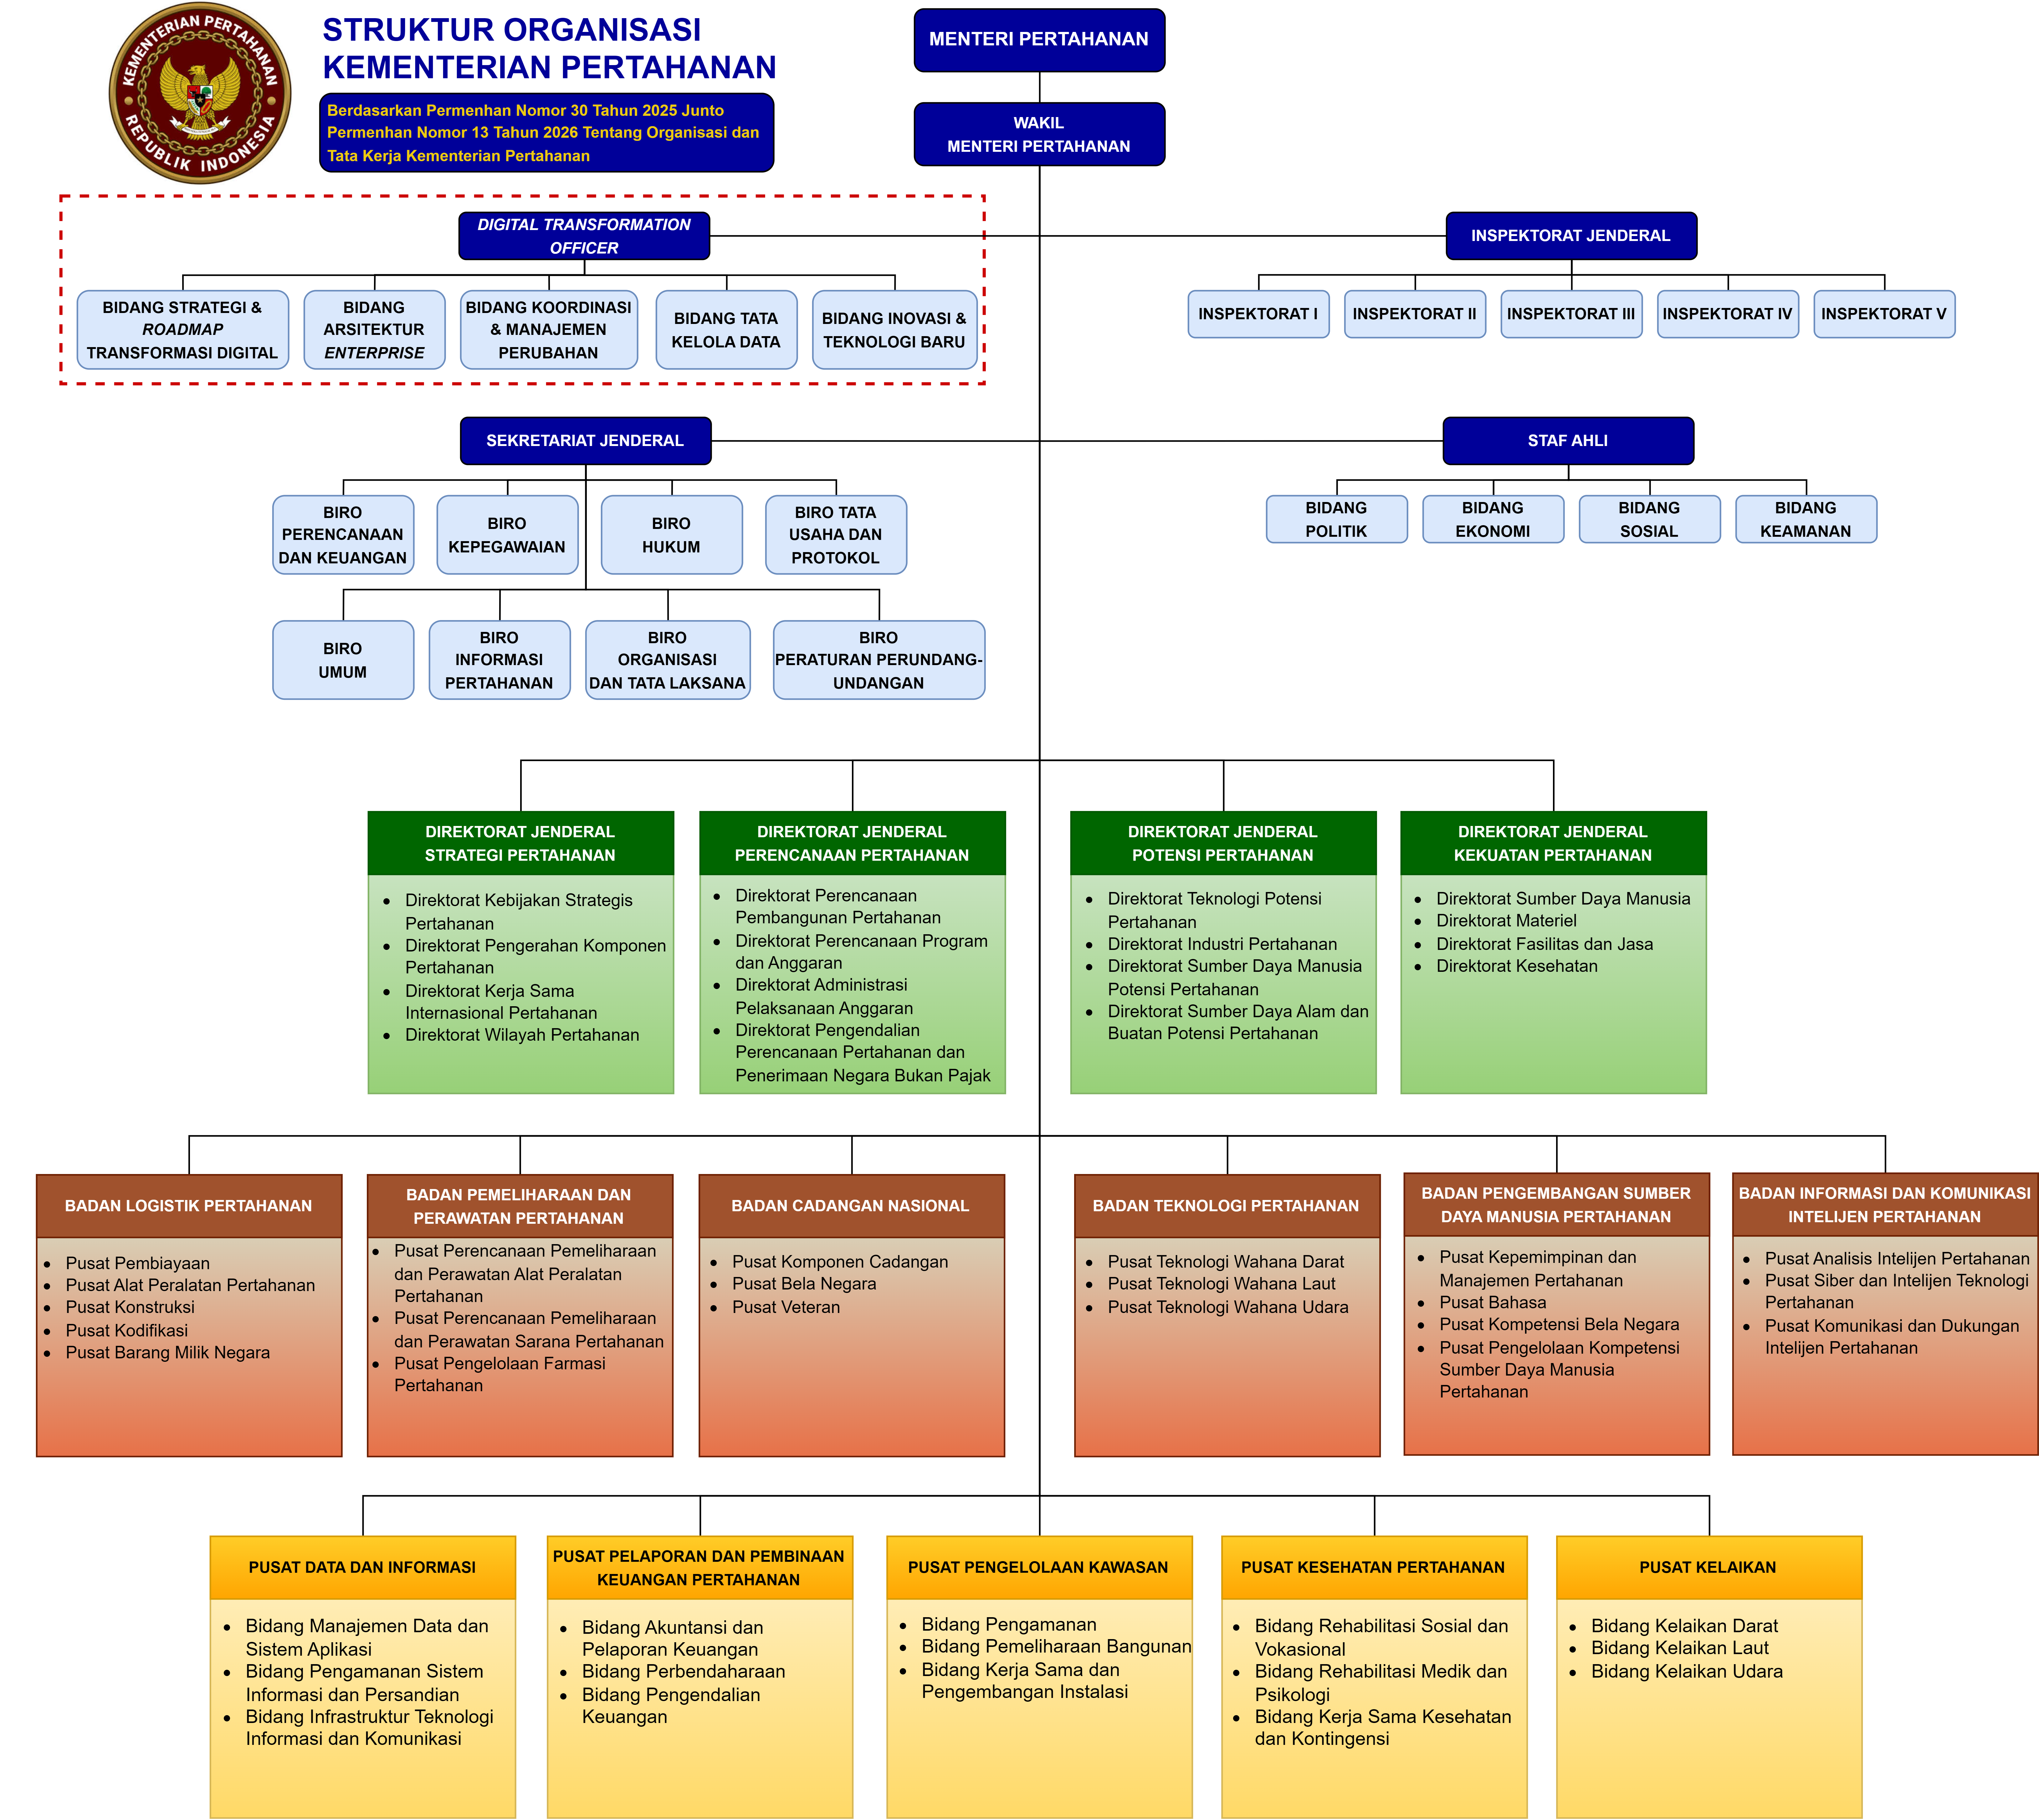
\includegraphics[width=0.9\textwidth]{images/Struktur Organisasi Kemhan Permenhan 30_2025 dan 13_2026 To Be.drawio.png}
\end{figure}

Unit DTO dipimpin oleh seorang \textit{Chief Digital Transformation Officer} yang sekaligus berperan sebagai \textit{Chief Enterprise Architect} dan memimpin \textit{Architecture Board}. Unit ini terdiri atas bidang-bidang berikut:
\begin{enumerate}[a.]
\item Bidang Strategi dan \textit{roadmap} Transformasi Digital, yang merumuskan strategi dan peta jalan (\textit{roadmap}) transformasi digital pertahanan;
\item Bidang Arsitektur \textit{Enterprise}, yang menyelenggarakan tata kelola arsitektur \textit{enterprise} dan standardisasi sistem lintas unit dan lintas matra, yang berisi para arsitek tiap domain (bisnis, data, aplikasi, teknologi, dan C5ISR);
\item Bidang Koordinasi dan Manajemen Perubahan, yang mengoordinasikan pelaksanaan transformasi lintas satuan kerja dan lintas matra serta mengelola manajemen perubahan (\textit{change management});
\item Bidang Tata Kelola Data, yang menyelenggarakan tata kelola data sebagai aset strategis, mencakup kebijakan data, penetapan wali data, dan standar data;
\item Bidang Inovasi dan Teknologi Baru, yang menelaah serta menyiapkan adopsi teknologi baru (\textit{emerging technology}).
\end{enumerate}

Pembagian bidang tersebut menegaskan bahwa unit DTO berfokus pada orkestrasi transformasi (\textit{change-the-business}) dan bukan pada operasional teknologi informasi, yang tetap menjadi ranah Badan Informasi dan Komunikasi Pertahanan (\textit{run-the-engine}). Dengan struktur ini, setiap fungsi strategis transformasi digital memiliki pengampu yang jelas dan dapat dipertanggungjawabkan.

\subsubsection{Peta Kapabilitas \textit{To-Be}}

Peta kapabilitas target (\textit{to-be}) merupakan pemutakhiran atas peta kapabilitas kondisi saat ini (Gambar~\ref{fig:kapabilitas-baseline}) dengan menambahkan kapabilitas baru yang diperlukan untuk mewujudkan arsitektur bisnis target. Penambahan difokuskan pada kapabilitas manajemen yang bersifat lintas fungsi serta menjadi prasyarat keberhasilan transformasi digital, tetapi belum tersedia pada kondisi \textit{baseline}. Oleh karena bersifat lintas fungsi, seluruh kapabilitas baru ditempatkan pada lapis \textit{shared}, sebagaimana disajikan pada Gambar~\ref{fig:kapabilitas-tobe}.

\begin{figure}[htbp]
\centering
\caption{Peta Kapabilitas Target (\textit{To-Be})}
\label{fig:kapabilitas-tobe}
\includegraphics[width=0.72\textwidth]{images/Value Stream & Business Capability Map Kemhan To-Be.drawio.png}
\end{figure}

Gambar~\ref{fig:kapabilitas-tobe} memperlihatkan tiga penambahan kapabilitas pada lapis \textit{shared} yang ditandai dengan warna hijau. Pertama, kapabilitas Tata Kelola Arsitektur \textit{Enterprise}, yang mencakup manajemen arsitektur \textit{enterprise}, standardisasi dan integrasi sistem, serta \textit{architecture governance} melalui \textit{Architecture Board}. Kapabilitas ini menjaga konsistensi rancangan sistem di seluruh aliran nilai sehingga tidak terikat pada satu \textit{value stream} tertentu. Kedua, kapabilitas Manajemen Perubahan, yang meliputi manajemen perubahan organisasi, adopsi dan komunikasi perubahan, serta kesiapan transformasi; kapabilitas ini menopang keberhasilan adopsi transformasi pada seluruh unit dan karenanya bersifat lintas organisasi. Ketiga, sub-kapabilitas Manajemen Talenta Digital yang disisipkan ke dalam kelompok Manajemen Sumber Daya Manusia untuk membedakannya dari manajemen talenta pertahanan yang telah ada pada lapis \textit{defining}, dengan penambahan ini menegaskan kebutuhan kompetensi digital yang berlaku menyeluruh di lingkungan organisasi.

Ketiga kapabilitas tersebut secara langsung merupakan kapabilitas pada bidang-bidang di dalam unit \textit{Digital Transformation Officer} (DTO), yaitu Bidang Arsitektur \textit{Enterprise}, Bidang Koordinasi dan Manajemen Perubahan, serta dukungan pengembangan talenta digital. Penempatannya pada lapis \textit{shared} menegaskan bahwa ketiganya merupakan kapabilitas manajemen berskala \textit{enterprise} yang diampu oleh fungsi bermandat lintas organisasi. Kelengkapan kapabilitas pada peta target inilah yang menjadi dasar identifikasi kesenjangan arsitektur bisnis.

\subsubsection{Analisis Kesenjangan}

Analisis kesenjangan (\textit{gap analysis}) membandingkan kondisi \textit{baseline} (\textit{as-is}) dengan arsitektur bisnis target (\textit{to-be}) untuk mengidentifikasi selisih yang harus ditutup. Hasil analisis disajikan pada Tabel~\ref{tab:gap-bisnis}.

\begin{longtable}{@{}p{0.04\textwidth}p{0.16\textwidth}p{0.24\textwidth}p{0.24\textwidth}p{0.22\textwidth}@{}}
\caption{Analisis Kesenjangan Arsitektur Bisnis}
\label{tab:gap-bisnis}\\
\toprule
\textbf{No.} & \textbf{Aspek Bisnis} & \textbf{Kondisi \textit{Baseline} (\textit{As-Is})} & \textbf{Kondisi Target (\textit{To-Be})} & \textbf{Kesenjangan dan Tindak Lanjut}\\
\midrule
\endfirsthead
\multicolumn{5}{c}{\tablename\ \thetable\ (lanjutan)}\\
\toprule
\textbf{No.} & \textbf{Aspek Bisnis} & \textbf{Kondisi \textit{Baseline} (\textit{As-Is})} & \textbf{Kondisi Target (\textit{To-Be})} & \textbf{Kesenjangan dan Tindak Lanjut}\\
\midrule
\endhead
\bottomrule
\endfoot
1 & Struktur dan mandat transformasi & Belum ada unit yang memegang mandat transformasi digital lintas organisasi & Fungsi DTO pada tingkat strategis dengan struktur internal yang jelas & Pembentukan unit DTO beserta bidang-bidangnya\\
\addlinespace
2 & Kapabilitas tata kelola arsitektur & Belum ada kapabilitas tata kelola arsitektur \textit{enterprise} dan standardisasi lintas unit & Kapabilitas \textit{Enterprise Architecture} dan \textit{Architecture Board} yang melekat pada DTO & Penetapan tata kelola dan standar arsitektur\\
\addlinespace
3 & Kapabilitas manajemen perubahan & Transformasi berjalan parsial tanpa pengelolaan perubahan & Kapabilitas manajemen perubahan (\textit{change management}) yang terlembaga & Pembangunan kapabilitas manajemen perubahan\\
\addlinespace
4 & Proses bisnis lintas unit & Proses bisnis terfragmentasi dan belum terstandar antarunit & Proses bisnis terstandar dan terintegrasi berbasis kapabilitas & Standardisasi dan integrasi proses bisnis\\
\addlinespace
5 & Koordinasi dan kolaborasi lintas matra & Koordinasi antarunit dan antarmatra bersifat \textit{ad hoc} & Mekanisme koordinasi transformasi lintas matra yang terlembaga & Penetapan mekanisme koordinasi lintas matra\\
\addlinespace
6 & Kompetensi dan talenta digital & Kompetensi digital terbatas dan tersebar antarunit & Kapabilitas manajemen talenta digital yang memadai & Program pengembangan dan rekrutmen talenta digital\\
\end{longtable}

\subsubsection{\textit{Roadmap} Implementasi}

\textit{Roadmap} implementasi fase \textit{business architecture} disusun berdasarkan urutan pelaksanaan inisiatif untuk menutup kesenjangan arsitektur bisnis pada Tabel~\ref{tab:gap-bisnis}. \textit{Roadmap} implementasi dibagi ke dalam tiga bagian waktu sebagaimana disajikan pada Gambar~\ref{fig:roadmap-bisnis} dan dirinci pada Tabel~\ref{tab:roadmap-bisnis}.

\begin{figure}[htbp]
\centering
\caption{\textit{Roadmap} Implementasi Fase \textit{Business Architecture}}
\label{fig:roadmap-bisnis}
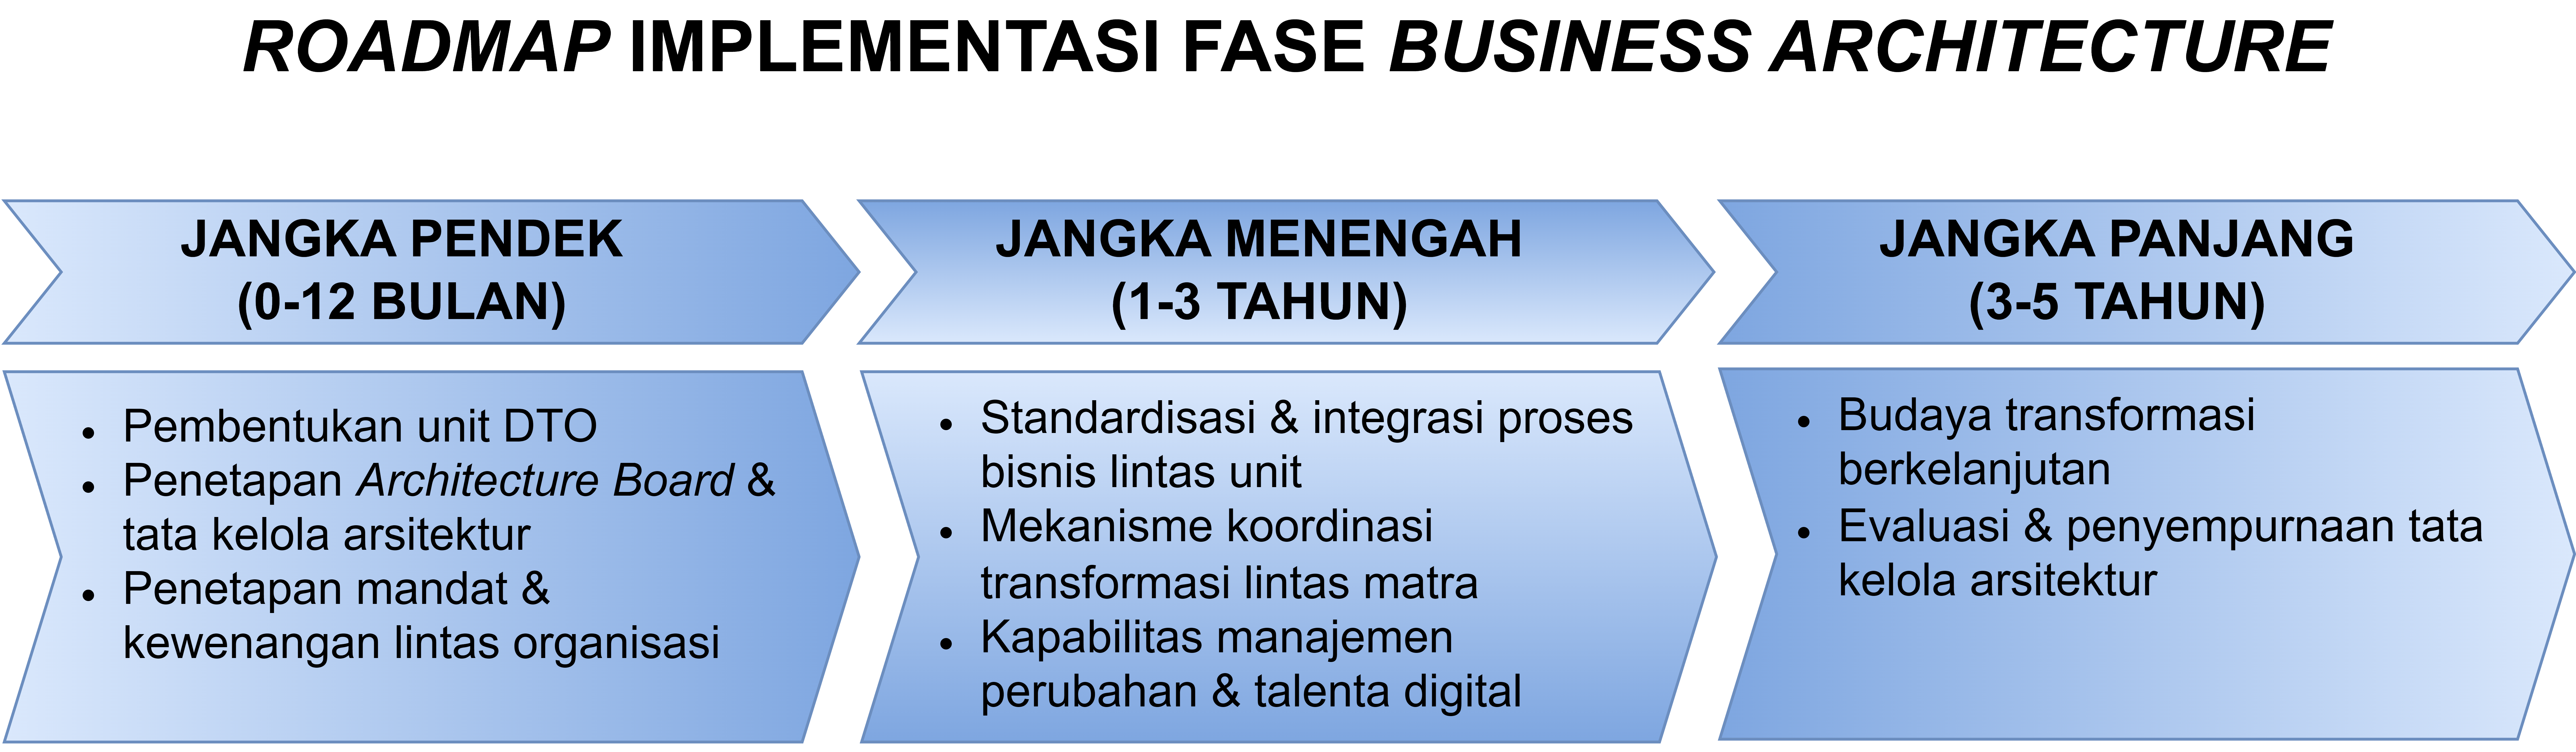
\includegraphics[width=0.9\textwidth]{images/Roadmap implementasi fase business architecture.drawio.png}
\end{figure}

\begin{longtable}{@{}p{0.20\textwidth}p{0.38\textwidth}p{0.35\textwidth}@{}}
\caption{Rincian \textit{Roadmap} Implementasi Fase \textit{Business}}
\label{tab:roadmap-bisnis}\\
\toprule
\textbf{Horizon Waktu} & \textbf{Inisiatif Bisnis} & \textbf{Keluaran dan Kesenjangan yang Ditutup}\\
\midrule
\endfirsthead
\multicolumn{3}{c}{\tablename\ \thetable\ (lanjutan)}\\
\toprule
\textbf{Horizon Waktu} & \textbf{Inisiatif Bisnis} & \textbf{Keluaran dan Kesenjangan yang Ditutup}\\
\midrule
\endhead
\bottomrule
\endfoot
Jangka Pendek (0--12 bulan) & Pembentukan unit DTO beserta bidang-bidangnya; penetapan \textit{Architecture Board} dan tata kelola arsitektur; penetapan mandat dan kewenangan lintas organisasi & Unit DTO operasional dan tata kelola arsitektur berjalan (menutup kesenjangan 1 dan 2)\\
\addlinespace
Jangka Menengah (1--3 tahun) & Standardisasi dan integrasi proses bisnis lintas unit; penetapan mekanisme koordinasi transformasi lintas matra; pembangunan kapabilitas manajemen perubahan dan talenta digital & Proses terstandar, koordinasi lintas matra terlembaga, serta kapabilitas perubahan dan talenta (menutup kesenjangan 3, 4, 5, dan 6)\\
\addlinespace
Jangka Panjang (3--5 tahun) & Pembentukan budaya transformasi berkelanjutan; evaluasi dan penyempurnaan tata kelola arsitektur & Organisasi berbasis kapabilitas yang matang dan berkelanjutan\\
\end{longtable}

Dengan demikian, fase \textit{Business Architecture} menghasilkan fondasi organisasi dan tata kelola yang menjadi prasyarat bagi keberhasilan transformasi pada fase-fase teknis berikutnya.


\section{Fase \textit{Information System Architecture}}

Fase \emph{Information Systems Architecture} menentukan arsitektur
sistem informasi yang mendukung proses bisnis pertahanan, mencakup
arsitektur data (\emph{data architecture}) dan arsitektur aplikasi
(\emph{application architecture}) yang dikerjakan berurutan dengan
arsitektur data didahulukan. Arsitektur data dirancang berdasarkan
Peraturan Presiden Nomor 39 Tahun 2019 tentang Satu Data Indonesia dan
Peraturan Menteri Pertahanan Nomor 1 Tahun 2023 tentang Satu Data
Pertahanan, sehingga penataan data pertahanan selaras dengan kebijakan
tata kelola data nasional maupun sektor pertahanan.

Kedua sub-domain arsitektur sistem informasi bermula dari inventarisasi
aplikasi Kemhan tahun 2025 yang menjadi kondisi \emph{baseline} bersama.
Oleh karena rekapitulasi ini digunakan baik oleh arsitektur data maupun
arsitektur aplikasi, rekapitulasi aplikasi \emph{baseline} per satuan
kerja disajikan pada Tabel~\ref{tab:iv-12}. Inventaris mencatat 247 aplikasi yang
terdiri atas 176 aplikasi umum dan 71 aplikasi khusus.

\begin{longtable}[]{@{}
  >{\raggedright\arraybackslash}p{\dimexpr 0.1176\columnwidth-2\tabcolsep\relax}
  >{\raggedright\arraybackslash}p{\dimexpr 0.4235\columnwidth-2\tabcolsep\relax}
  >{\raggedright\arraybackslash}p{\dimexpr 0.1294\columnwidth-2\tabcolsep\relax}
  >{\raggedright\arraybackslash}p{\dimexpr 0.1529\columnwidth-2\tabcolsep\relax}
  >{\raggedright\arraybackslash}p{\dimexpr 0.1529\columnwidth-2\tabcolsep\relax}@{}}
\caption{Rekapitulasi Aplikasi \textit{Baseline} per Satuan Kerja}\label{tab:iv-12}\\
\toprule\noalign{}
\begin{minipage}[b]{\linewidth}\raggedright
\textbf{No.}
\end{minipage} & \begin{minipage}[b]{\linewidth}\raggedright
\textbf{Satuan Kerja}
\end{minipage} & \begin{minipage}[b]{\linewidth}\raggedright
\textbf{Umum}
\end{minipage} & \begin{minipage}[b]{\linewidth}\raggedright
\textbf{Khusus}
\end{minipage} & \begin{minipage}[b]{\linewidth}\raggedright
\textbf{Jumlah}
\end{minipage} \\
\midrule\noalign{}
\endhead
\bottomrule\noalign{}
\endlastfoot
1 & Direktorat Jenderal Strategi Pertahanan & 10 & 0 & 10 \\
2 & Direktorat Jenderal Perencanaan Pertahanan & 22 & 0 & 22 \\
3 & Direktorat Jenderal Potensi Pertahanan & 8 & 4 & 12 \\
4 & Direktorat Jenderal Kekuatan Pertahanan & 21 & 0 & 21 \\
5 & Inspektorat Jenderal & 2 & 1 & 3 \\
6 & Biro Perencanaan dan Keuangan & 2 & 0 & 2 \\
7 & Biro Kepegawaian & 2 & 4 & 6 \\
8 & Biro Hukum & 0 & 1 & 1 \\
9 & Biro Tata Usaha dan Protokol & 16 & 0 & 16 \\
10 & Biro Umum & 17 & 0 & 17 \\
11 & Biro Informasi Pertahanan & 0 & 2 & 2 \\
12 & Biro Organisasi dan Tata Laksana & 0 & 1 & 1 \\
13 & Biro Peraturan Perundang-undangan & 1 & 0 & 1 \\
14 & Badan Logistik Pertahanan & 5 & 1 & 6 \\
15 & Badan Teknologi Pertahanan & 18 & 1 & 19 \\
16 & Badan Pengembangan Sumber Daya Manusia Pertahanan & 0 & 27 & 27 \\
17 & Pusat Data dan Informasi & 6 & 8 & 14 \\
18 & Badan Informasi dan Komunikasi Intelijen Pertahanan & 0 & 16 &
16 \\
19 & Pusat Kelaikan & 13 & 0 & 13 \\
20 & Pusat Kesehatan Pertahanan & 14 & 4 & 18 \\
21 & Pusat Pelaporan dan Pembinaan Keuangan Pertahanan & 12 & 1 & 13 \\
22 & Universitas Pertahanan & 7 & 0 & 7 \\
& \textbf{Total} & \textbf{176} & \textbf{71} & \textbf{247} \\
\end{longtable}

\subsection{Data Architecture}

Arsitektur data merancang struktur definisi, klasifikasi, dan tata
kelola kepemilikan Data Pertahanan. Mengacu Permenhan Nomor 1 Tahun
2023, \emph{Data Pertahanan} adalah data yang dibina dan diselenggarakan
oleh Kementerian Pertahanan dan Tentara Nasional Indonesia untuk
kepentingan penyelenggaraan pertahanan negara. Perancangan berpedoman
pada prinsip \emph{Data as Strategic Asset} serta empat prinsip Satu
Data Indonesia, yaitu pemenuhan standar data, metadata, kaidah
interoperabilitas data, dan penggunaan kode referensi serta data induk.

\subsubsection{Arsitektur Data \textit{Baseline}}

Arsitektur data \emph{baseline} diturunkan dari inventarisasi aplikasi
Kemhan tahun 2025 yang mencatat 247 aplikasi, terdiri atas 176 aplikasi
umum dan 71 aplikasi khusus. Aplikasi umum merupakan sistem nasional
yang digunakan bersama oleh banyak instansi seperti: SAKTI, SIMPEG,
SIRUP, KRISNA, dan OM-SPAN, sehingga Kemhan berkedudukan sebagai
pengguna, bukan pemilik datanya. Data pada aplikasi umum tunduk pada
tata kelola instansi penyelenggara masing-masing di tingkat nasional dan
karenanya berada di luar lingkup arsitektur data Kemhan. Sebaliknya,
aplikasi khusus merupakan aplikasi yang dibina dan diselenggarakan
sendiri oleh Kemhan, sehingga datanya merupakan Data Pertahanan dan
menjadi lingkup utama arsitektur data serta Satu Data Pertahanan.

\subsubsection{Model Entitas Data Pertahanan}

Model entitas data menggambarkan objek data pokok (entitas) yang menjadi
rujukan proses bisnis pertahanan beserta sumber dan pengelolanya.
Entitas data diturunkan dari fungsi 71 aplikasi khusus yang menghasilkan
Data Pertahanan, kemudian dikelompokkan menurut kedekatan domainnya,
yaitu domain kepegawaian, hukum, dan pengawasan; layanan publik dan
potensi pertahanan; pendidikan, kesehatan, litbang, dan keuangan; serta
data strategis, geospasial, dan keamanan siber. Daftar entitas data
utama Data Pertahanan disajikan pada Tabel~\ref{tab:iv-13}.

\begin{longtable}[]{@{}
  >{\raggedright\arraybackslash}p{\dimexpr 0.1954\columnwidth-2\tabcolsep\relax}
  >{\raggedright\arraybackslash}p{\dimexpr 0.2299\columnwidth-2\tabcolsep\relax}
  >{\raggedright\arraybackslash}p{\dimexpr 0.2299\columnwidth-2\tabcolsep\relax}
  >{\raggedright\arraybackslash}p{\dimexpr 0.3218\columnwidth-2\tabcolsep\relax}@{}}
\caption{Entitas Data Pertahanan}\label{tab:iv-13}\\
\toprule\noalign{}
\begin{minipage}[b]{\linewidth}\raggedright
\textbf{No.}
\end{minipage} & \begin{minipage}[b]{\linewidth}\raggedright
\textbf{Entitas Data}
\end{minipage} & \begin{minipage}[b]{\linewidth}\raggedright
\textbf{Aplikasi}
\end{minipage} & \begin{minipage}[b]{\linewidth}\raggedright
\textbf{Deskripsi}
\end{minipage} \\
\midrule\noalign{}
\endhead
\bottomrule\noalign{}
\endlastfoot
\textbf{Kepegawaian, Hukum, dan Pengawasan} & & & \\
1 & Data Kinerja Pegawai & E-Kinerja, E-LAPKIN & Capaian dan laporan
kinerja pegawai serta kinerja organisasi \\
2 & Data Kompetensi \& Asesmen & SIAC & Hasil asesmen kompetensi dan
pemetaan talenta pegawai \\
3 & Data Kartu Identitas Pegawai & E-KTA, SiUdin & Identitas resmi dan
kartu tanda anggota pegawai \\
4 & Data Perkara \& Dokumentasi Hukum & Si Rokum & Perkara, pendapat
hukum, dan dokumentasi produk hukum \\
5 & Data Pengawasan Intern & SIMWAS & Temuan, rekomendasi, dan tindak
lanjut hasil pengawasan intern \\
\textbf{Layanan Publik dan Potensi Pertahanan} & & & \\
6 & Data Layanan Informasi Publik & E-PPID, Smart Mobile Reporting &
Permohonan informasi publik \\
7 & Data Veteran & Veteran & Identitas, status, dan hak-hak veteran
pertahanan negara \\
8 & Data Sumber Daya \& Industri Pertahanan & Sisinfo Sumdahan, Daya
Serap & Potensi sumber daya nasional dan kapasitas industri
pertahanan \\
9 & Data Perizinan Pertahanan & Perizinan & Permohonan dan penerbitan
izin di bidang industri pertahanan \\
\textbf{Pendidikan, Kesehatan, Litbang, dan Keuangan} & & & \\
10 & Data Peserta Didik \& Akademik & Aplikasi Pengelolaan
Siswa/Akademik, Sistem Layanan Diklat & Peserta didik, kurikulum,
jadwal, dan nilai akademik \\
11 & Data Alumni & Sistem Pengelolaan Alumni & Riwayat dan penelusuran
alumni pendidikan pertahanan \\
12 & Data Bahan Ajar \& Pembelajaran Digital & Bahan Ajar Digital, VR
Diklat, Sistem Pembelajaran Elektronik & Materi ajar, modul, dan konten
pembelajaran digital \\
13 & Data Rekam Medis \& Pasien & SimRS, Sismadak & Rekam medis, riwayat
layanan, dan mutu pelayanan pasien \\
14 & Data Klaim Layanan Kesehatan & E-Klaim & Pengajuan dan verifikasi
klaim layanan kesehatan \\
15 & Data Penelitian \& Pengembangan & Data Digital Arsip Penelitian &
Arsip hasil penelitian dan pengembangan pertahanan \\
16 & Data Pelaporan Keuangan Internal & EMINU & Pelaporan dan pemantauan
keuangan internal Kemhan \\
\textbf{Data Strategis, Geospasial, dan Keamanan Siber} & & & \\
17 & Data Geospasial Wilayah Pertahanan & Peta Tematik Wilayah
Pertahanan, Layanan Peta Digital, IGD Sumdahan & Peta tematik dan data
spasial wilayah serta objek pertahanan \\
18 & Data Log \& Insiden Keamanan Siber & SIEM, Splunk, Honeypot, Log
Manajemen & Catatan aktivitas, deteksi, dan penanganan insiden keamanan
siber \\
19 & Data Identitas \& Kendali Akses & Single Sign On (SSO), Access
Control & Identitas pengguna, hak akses, dan otentikasi sistem \\
20 & Data Aset \& Infrastruktur TIK & Rack Management, EMS, The Dude,
Cacti & Inventaris dan kondisi perangkat, jaringan, serta infrastruktur
TIK \\
\end{longtable}

\subsubsection{Klasifikasi Data menurut Tingkat Kerahasiaan}

Klasifikasi data menurut tingkat kerahasiaan diperlukan untuk
menyeimbangkan kewajiban berbagi-pakai data dengan kewajiban kerahasiaan
pertahanan. Mengacu pada Permenhan Nomor 1 Tahun 2023 tentang Satu Data
Pertahanan Pasal 21, klasifikasi Data Pertahanan terdiri atas tiga
tingkat, yaitu Klasifikasi Data Terbuka, Klasifikasi Data Terbatas, dan
Klasifikasi Data Rahasia, sebagaimana disajikan pada Tabel~\ref{tab:iv-14}.

\begin{longtable}[]{@{}
  >{\raggedright\arraybackslash}p{\dimexpr 0.2338\columnwidth-2\tabcolsep\relax}
  >{\raggedright\arraybackslash}p{\dimexpr 0.4026\columnwidth-2\tabcolsep\relax}
  >{\raggedright\arraybackslash}p{\dimexpr 0.3377\columnwidth-2\tabcolsep\relax}@{}}
\caption{Klasifikasi Data Pertahanan}\label{tab:iv-14}\\
\toprule\noalign{}
\begin{minipage}[b]{\linewidth}\raggedright
\textbf{Klasifikasi}
\end{minipage} & \begin{minipage}[b]{\linewidth}\raggedright
\textbf{Kriteria}
\end{minipage} & \begin{minipage}[b]{\linewidth}\raggedright
\textbf{Kendali Akses}
\end{minipage} \\
\midrule\noalign{}
\endhead
\bottomrule\noalign{}
\endlastfoot
Data Terbuka & Data yang diperbolehkan untuk diketahui publik & Terbuka
untuk publik melalui Portal Satu Data Pertahanan \\
Data Terbatas & Data yang hanya dapat diakses oleh kementerian/lembaga
yang diberikan akses oleh Walidata Pertahanan & Otentikasi dan hak akses
berbasis izin oleh Walidata Pertahanan \\
Data Rahasia & Data yang hanya dapat diakses oleh pejabat berwenang di
Kemhan, Markas Besar TNI, dan Markas Besar Angkatan & Otorisasi khusus,
enkripsi, dan pencatatan audit \\
\end{longtable}

\subsubsection{Kamus Data dan Standar Penamaan}

Kamus data (\emph{data dictionary}) dan standar penamaan disusun untuk
memenuhi prinsip Satu Data Indonesia dan Satu Data Pertahanan, yaitu
pemenuhan standar data, metadata, kaidah interoperabilitas, serta
penggunaan kode referensi dan data induk. Tanpa definisi dan penamaan
yang seragam, entitas data yang sama dapat direkam berbeda antaraplikasi
khusus sehingga menghambat interoperabilitas. Standar penamaan yang
ditetapkan sebagai berikut:

\begin{quote}
a. nama entitas dan atribut menggunakan bahasa Indonesia baku,
deskriptif, dan tidak memakai singkatan yang ambigu;

b. penamaan atribut mengikuti pola {[}entitas{]}\_{[}atribut{]} dengan
huruf kecil dan pemisah garis bawah (\emph{snake\_case}), misalnya
pegawai\_nip dan veteran\_nomor;

c. setiap entitas memiliki satu pengidentifikasi unik (\emph{primary
key}) yang baku, misalnya NIP/NRP untuk pegawai dan nomor registrasi
untuk veteran;

d. setiap entitas dan atribut memiliki definisi tunggal yang disepakati
dan dicatat dalam kamus data; dan

e. metadata mengikuti struktur dan format baku Satu Data Indonesia,
mencakup definisi, format, satuan, klasifikasi, dan wali data.
\end{quote}

\subsubsection{Matriks Kepemilikan dan Tata Kelola Data}

Tata kelola Data Pertahanan mengikuti penyelenggara Satu Data Pertahanan
sebagaimana ditetapkan Permenhan Nomor 1 Tahun 2023. Penetapan peran
yang jelas menjamin setiap Data Pertahanan memiliki produsen dan wali
data yang bertanggung jawab atas mutunya. Peran-peran tersebut disajikan
pada Tabel~\ref{tab:iv-15}.

\begin{longtable}[]{@{}
  >{\raggedright\arraybackslash}p{\dimexpr 0.2297\columnwidth-2\tabcolsep\relax}
  >{\raggedright\arraybackslash}p{\dimexpr 0.4324\columnwidth-2\tabcolsep\relax}
  >{\raggedright\arraybackslash}p{\dimexpr 0.3108\columnwidth-2\tabcolsep\relax}@{}}
\caption{Peran Penyelenggaraan Satu Data Pertahanan}\label{tab:iv-15}\\
\toprule\noalign{}
\begin{minipage}[b]{\linewidth}\raggedright
\textbf{Peran}
\end{minipage} & \begin{minipage}[b]{\linewidth}\raggedright
\textbf{Tugas Pokok}
\end{minipage} & \begin{minipage}[b]{\linewidth}\raggedright
\textbf{Pemangku Peran}
\end{minipage} \\
\midrule\noalign{}
\endhead
\bottomrule\noalign{}
\endlastfoot
Pengarah & Mengoordinasikan pelaksanaan, pemantauan, evaluasi, dan
pelaporan Satu Data Pertahanan kepada Menteri & Sekretaris Jenderal
Kemhan \\
Walidata Pertahanan & Merencanakan, mengumpulkan, memeriksa, mengelola,
dan menyebarluaskan data melalui Portal Satu Data Pertahanan & Pusat
Data dan Informasi \\
Produsen Data Pertahanan & Menghasilkan data sesuai prinsip Satu Data
serta menyampaikan data dan metadata kepada Walidata & Satuan kerja
penghasil data di lingkungan Kemhan dan Mabes TNI \\
Pengolah Data Pertahanan & Mendistribusikan Data Pertahanan hingga
sampai kepada Walidata & Satuan kerja pengelola data di Mabes
Angkatan \\
Pengaman Sistem Data Pertahanan & Mengamankan, memantau, menguji, dan
merespons ancaman siber terhadap sistem Satu Data Pertahanan & Bidang
Pengamanan Sistem Informasi dan Persandian pada Pusat Data dan
Informasi, didukung Pusat Siber dan Intelijen Teknologi Pertahanan
Pertahanan \\
Forum Satu Data Pertahanan & Wadah komunikasi dan koordinasi
penyelenggaraan Satu Data Pertahanan & Walidata, Produsen, Pengolah, dan
Pengaman Sistem Data \\
\end{longtable}

Berdasarkan pembagian peran tersebut, setiap Data Pertahanan memiliki
produsen data (satuan kerja) sebagai penghasil, sedangkan pengelolaan
dan penyebarluasannya dipusatkan pada satu Walidata Pertahanan, yaitu
Pusat Data dan Informasi yang menyelenggarakan manajemen Satu Data
Pertahanan sesuai Permenhan Nomor 30 Tahun 2025 sebagaimana diubah
dengan Permenhan Nomor 13 Tahun 2026.

\subsubsection{Arsitektur Data Target}

Arsitektur data target adalah terwujudnya Satu Data Pertahanan, yaitu
Data Pertahanan yang terstandar, terklasifikasi, dimiliki secara jelas,
aman, dan dapat dibagipakaikan secara terkendali. Sarana teknis
pewujudannya adalah Portal Satu Data Pertahanan, yaitu media bagi-pakai
data yang dikelola Walidata Pertahanan dan terhubung dengan Portal Satu
Data Indonesia. Arsitektur data target dibangun di atas lima komponen
berikut:

\begin{quote}
a. Kamus data dan standar penamaan sebagai rujukan tunggal definisi,
penamaan, dan metadata;

b. Klasifikasi dan kendali akses yang menetapkan tingkat kerahasiaan dan
hak akses;

c. Tata kelola dan wali data sesuai penyelenggara Satu Data Pertahanan;

d. Portal Satu Data Pertahanan sebagai platform bagi-pakai dan
penyebarluasan data, dilengkapi kode referensi dan data induk;

e. Interoperabilitas data dengan Portal Satu Data Indonesia sesuai
kaidah Satu Data Indonesia.
\end{quote}

\subsubsection{Analisis Kesenjangan}

Analisis kesenjangan (\emph{gap analysis}) membandingkan kondisi
arsitektur data \emph{baseline} (\emph{as-is}) dengan arsitektur data
target (\emph{to-be}) untuk mengidentifikasi selisih yang harus ditutup
beserta tindak lanjutnya. Analisis difokuskan pada enam aspek utama Data
Pertahanan, yaitu standar dan definisi data, integrasi dan
berbagi-pakai, tata kelola dan kepemilikan, klasifikasi kerahasiaan,
keamanan dan akses, serta interoperabilitas. Perbandingan ketiga kondisi
tersebut disajikan pada Tabel~\ref{tab:iv-16}.

\begin{longtable}[]{@{}
  >{\raggedright\arraybackslash}p{\dimexpr 0.1111\columnwidth-2\tabcolsep\relax}
  >{\raggedright\arraybackslash}p{\dimexpr 0.2222\columnwidth-2\tabcolsep\relax}
  >{\raggedright\arraybackslash}p{\dimexpr 0.2000\columnwidth-2\tabcolsep\relax}
  >{\raggedright\arraybackslash}p{\dimexpr 0.2222\columnwidth-2\tabcolsep\relax}
  >{\raggedright\arraybackslash}p{\dimexpr 0.2222\columnwidth-2\tabcolsep\relax}@{}}
\caption{Analisis Kesenjangan Arsitektur Data Pertahanan}\label{tab:iv-16}\\
\toprule\noalign{}
\begin{minipage}[b]{\linewidth}\raggedright
\textbf{No.}
\end{minipage} & \begin{minipage}[b]{\linewidth}\raggedright
\textbf{Aspek}
\end{minipage} & \begin{minipage}[b]{\linewidth}\raggedright
\textbf{Baseline (As-Is)}
\end{minipage} & \begin{minipage}[b]{\linewidth}\raggedright
\textbf{Target (To-Be)}
\end{minipage} & \begin{minipage}[b]{\linewidth}\raggedright
\textbf{Kesenjangan dan Tindak Lanjut}
\end{minipage} \\
\midrule\noalign{}
\endhead
\bottomrule\noalign{}
\endlastfoot
1 & Standar dan definisi data & Definisi dan penamaan berbeda
antaraplikasi khusus & Kamus data dan standar penamaan yang seragam &
Penetapan dan penerapan kamus data serta standar penamaan \\
2 & Integrasi dan berbagi-pakai & Data Pertahanan terkotak (silo) per
aplikasi dan satker & Berbagi-pakai melalui Portal Satu Data Pertahanan
& Pembangunan Portal Satu Data Pertahanan \\
3 & Tata kelola dan kepemilikan & Belum ada wali data dan produsen data
yang baku & Walidata Pertahanan dan produsen data sesuai Permenhan
1/2023 & Penetapan penyelenggara Satu Data Pertahanan \\
4 & Klasifikasi kerahasiaan & Belum ada klasifikasi yang tegas & Tiga
tingkat klasifikasi (Terbuka, Terbatas, Rahasia) & Penetapan dan
penerapan klasifikasi data \\
5 & Keamanan dan akses & Kendali akses parsial per aplikasi & Kendali
akses berbasis klasifikasi dan pengamanan sistem & Penerapan kendali
akses dan pengaman sistem data \\
6 & Interoperabilitas & Pertukaran data manual/terbatas &
Interoperabilitas dengan Portal Satu Data Indonesia & Penetapan kode
referensi, data induk, dan kaidah interoperabilitas \\
\end{longtable}

\subsection{Application Architecture}

Arsitektur aplikasi merancang portofolio aplikasi yang mendukung proses
bisnis pertahanan, mencakup aplikasi yang digunakan, fungsi yang
didukung, pengguna, serta keterhubungan (integrasi) antaraplikasi.
Sesuai lingkup yang ditetapkan pada arsitektur data, arsitektur aplikasi
difokuskan pada 71 aplikasi khusus yang dibina dan diselenggarakan
sendiri oleh Kemhan.

\subsubsection{Arsitektur Aplikasi \textit{Baseline}}

Arsitektur aplikasi \emph{baseline} menggambarkan 71 aplikasi khusus
yang digunakan Kemhan pada tahun 2025 beserta uraian dan penggunanya.
Aplikasi dikelompokkan menurut domain agar mudah diteliti. Daftar
aplikasi khusus disajikan pada Tabel~\ref{tab:iv-17}

\begin{longtable}[]{@{}
  >{\raggedright\arraybackslash}p{\dimexpr 0.2045\columnwidth-2\tabcolsep\relax}
  >{\raggedright\arraybackslash}p{\dimexpr 0.2159\columnwidth-2\tabcolsep\relax}
  >{\raggedright\arraybackslash}p{\dimexpr 0.3523\columnwidth-2\tabcolsep\relax}
  >{\raggedright\arraybackslash}p{\dimexpr 0.2045\columnwidth-2\tabcolsep\relax}@{}}
\caption{Daftar Aplikasi}\label{tab:iv-17}\\
\toprule\noalign{}
\begin{minipage}[b]{\linewidth}\raggedright
\textbf{No.}
\end{minipage} & \begin{minipage}[b]{\linewidth}\raggedright
\textbf{Aplikasi}
\end{minipage} & \begin{minipage}[b]{\linewidth}\raggedright
\textbf{Uraian}
\end{minipage} & \begin{minipage}[b]{\linewidth}\raggedright
\textbf{Pengguna}
\end{minipage} \\
\midrule\noalign{}
\endhead
\bottomrule\noalign{}
\endlastfoot
\textbf{Kepegawaian} & & & \\
1 & E-Kinerja & Pengelolaan rencana dan capaian kinerja pegawai & Biro
Kepegawaian \\
2 & SIAC & Pelayanan asesmen kompetensi pegawai & Biro Kepegawaian \\
3 & SiUdin & Pelayanan ujian dinas dan penyesuaian ijazah pegawai & Biro
Kepegawaian \\
4 & E-KTA & Pengajuan dan pencetakan Kartu Tanda Anggota & Biro
Kepegawaian \\
5 & E-LAPKIN & Pelaporan kinerja pegawai & Biro Ortala \\
\textbf{Hukum dan Pengawasan} & & & \\
6 & Si Rokum & Penatausahaan data penanganan perkara hukum & Biro
Hukum \\
7 & SIMWAS Ver 2.0 & Pengelolaan dokumen hasil pengawasan intern &
Inspektorat Jenderal \\
\textbf{Informasi Publik} & & & \\
8 & E-PPID & Penerimaan permohonan informasi publik & Biro Informasi
Pertahanan \\
9 & Smart Mobile Reporting & Pelaporan dan pemantauan perjalanan dinas &
Biro Informasi Pertahanan \\
\textbf{Potensi Pertahanan} & & & \\
10 & Perizinan & Layanan perizinan industri pertahanan daring & Ditjen
Potensi Pertahanan \\
11 & Veteran & Pelayanan administrasi keveteranan daring & Ditjen
Potensi Pertahanan \\
12 & Sisinfo Sumdahan & Manajemen sumber daya pertahanan (Komcad dan
Komduk) & Ditjen Potensi Pertahanan \\
13 & Daya Serap & Pemantauan daya serap program dan anggaran & Ditjen
Potensi Pertahanan \\
\textbf{Sarana Pertahanan} & & & \\
14 & Monitoring Dokumen Elektronik & Penyimpanan dan pencarian surat
secara digital & Badan Logistik Pertahanan \\
\textbf{Pendidikan dan Pelatihan} & & & \\
15 & Aplikasi Command Center & Pemantauan dan pusat kendali fasilitas
diklat & Badan Pengembangan Sumber Daya Manusia Pertahanan \\
16 & Virtual Collaboration System & Aplikasi berbasis web untuk
melakukan meeting di dunia maya & Badan Pengembangan Sumber Daya Manusia
Pertahanan \\
17 & Security Management System & Pengenalan wajah dan keamanan
fasilitas & Badan Pengembangan Sumber Daya Manusia Pertahanan \\
18 & Energy Management System & Pemantauan penggunaan listrik & Badan
Pengembangan Sumber Daya Manusia Pertahanan \\
19 & Access Management System & Pengelolaan data dan akses tamu & Badan
Pengembangan Sumber Daya Manusia Pertahanan \\
20 & Sistem Layanan Diklat & Layanan bantuan dan informasi diklat &
Badan Pengembangan Sumber Daya Manusia Pertahanan \\
21 & Bahan Ajar Digital Diklat & Pembelajaran bahan ajar secara digital
& Badan Pengembangan Sumber Daya Manusia Pertahanan \\
22 & VR Diklat Jemenhan & Bahan ajar manajemen pertahanan berbasis VR &
Badan Pengembangan Sumber Daya Manusia Pertahanan \\
23 & Simulasi Manajemen Pertahanan & Familiarisasi bahan ajar melalui
simulasi 3 dimensi & Badan Pengembangan Sumber Daya Manusia
Pertahanan \\
24 & Sistem Informasi Badiklat & Website untuk menyampaikan informasi
berkaitan dengan Badiklat dan Pusdiklat & Badan Pengembangan Sumber Daya
Manusia Pertahanan \\
25 & Sistem Pengelolaan Alumni & Pemantauan dan penelusuran data alumni
& Badan Pengembangan Sumber Daya Manusia Pertahanan \\
26 & Sistem Pemantauan \& Pengelolaan Sisfo Diklat & Pemantauan
perkembangan diklat & Badan Pengembangan Sumber Daya Manusia
Pertahanan \\
27 & Sistem Dasbor Pimpinan & Ringkasan kegiatan diklat bagi pimpinan &
Badan Pengembangan Sumber Daya Manusia Pertahanan \\
28 & VR Diklat Bahasa & Bahan ajar bahasa berbasis VR & Badan
Pengembangan Sumber Daya Manusia Pertahanan \\
29 & Lab Bahasa & Pembelajaran laboratorium bahasa & Badan Pengembangan
Sumber Daya Manusia Pertahanan \\
30 & Aplikasi Pengelolaan Siswa & Data dan pendaftaran siswa & Badan
Pengembangan Sumber Daya Manusia Pertahanan \\
31 & Aplikasi Pengelolaan Akademik & Aplikasi berbasis web yang
menyediakan layanan data siswa, pendaftaran online, ploting asrama,
lapor datang & Badan Pengembangan Sumber Daya Manusia Pertahanan \\
32 & Sistem Pengelolaan Aset & Pengelolaan aset dan inventaris internal
Tekfunghan & Badan Pengembangan Sumber Daya Manusia Pertahanan \\
33 & Ujian Berbasis Komputer & Layanan ujian berbasis komputer & Badan
Pengembangan Sumber Daya Manusia Pertahanan \\
34 & Kios Siswa & Informasi bagi siswa Tekfunghan & Badan Pengembangan
Sumber Daya Manusia Pertahanan \\
35 & Aplikasi Manajemen Pengajaran & Aplikasi berbasis web yang
menyediakan layanan jadwal pengajaran, rekapitulasi jam pelajaran
widyaiswara, catatan mengajar, perangkat mengajar, penjadwalan
widyaiswara & Badan Pengembangan Sumber Daya Manusia Pertahanan \\
36 & Sistem Konferensi Kelas & Pembelajaran jarak jauh (distance
learning) & Badan Pengembangan Sumber Daya Manusia Pertahanan \\
37 & VR Diklat Tekfunghan & Bahan ajar diklat Tekfunghan berbasis VR &
Badan Pengembangan Sumber Daya Manusia Pertahanan \\
38 & Bahan Ajar Digital Tekfunghan & Aplikasi berbasis desktop untuk
menampilkan materi pembelajaran secara interaktif di dalam kelas
Tekfunghan & Badan Pengembangan Sumber Daya Manusia Pertahanan \\
39 & Sistem Pembelajaran Elektronik & Pembelajaran daring dan tatap muka
& Badan Pengembangan Sumber Daya Manusia Pertahanan \\
40 & Bahan Ajar Digital Bela Negara & Pembelajaran bela negara di ruang
kelas & Badan Pengembangan Sumber Daya Manusia Pertahanan \\
41 & VR Diklat Bela Negara & Bahan ajar bela negara berbasis VR & Badan
Pengembangan Sumber Daya Manusia Pertahanan \\
\textbf{Kesehatan dan Rehabilitasi} & & & \\
42 & SimRS & Sistem informasi manajemen rumah sakit & Pusat Kesehatan
Pertahanan \\
43 & Sismadak & Manajemen dan akreditasi rumah sakit & Pusat Kesehatan
Pertahanan \\
44 & E-Klaim & Klaim layanan kesehatan secara elektronik & Pusat
Kesehatan Pertahanan \\
45 & Website RSPPN & Situs layanan dan informasi RSPPN & Pusat Kesehatan
Pertahanan \\
\textbf{Data Strategis dan Geospasial} & & & \\
46 & Big Data & Penyajian data media daring dan media sosial & Pusat
Data dan Informasi \\
47 & Program Kerja Pusdatin & Layanan Monitoring dan Koordinasi
Pelaksanaan Program Kerja Pusdatin & Pusat Data dan Informasi \\
48 & Pusdatin Cloud & Layanan penyimpanan dokumen dan file untuk pegawai
Pusdatin kemhan & Pusat Data dan Informasi \\
49 & IGD Sumdahan & Layanan untuk mendukungan Defense Strategic Room
Menteri Pertahanan & Pusat Data dan Informasi; pimpinan \\
50 & Secure Code Analyzer & Sistem yang digunakan untuk melakukan
scanning terhadap \emph{source code} aplikasi &
\begin{minipage}[t]{\linewidth}\raggedright
Pusat Data dan Informasi;\\
Bid. Sistem Aplikasi\strut
\end{minipage} \\
51 & Peta Tematik Wilayah Pertahanan & Penyajian peta pertahanan dan
titik strategis & Pusat Data dan Informasi \\
52 & Layanan Peta Digital & Analisis dan pemasangan titik (POI) pada
peta & Pusat Data dan Informasi \\
53 & SIMONAS & Pemantauan aplikasi dan server &
\begin{minipage}[t]{\linewidth}\raggedright
Pusat Data dan Informasi;\\
Bid. Infra TIK\strut
\end{minipage} \\
\textbf{Keamanan Siber dan Infrastruktur TIK} & & & \\
54 & The Dude & Pemantauan kondisi perangkat jaringan & Badan Informasi
dan Komunikasi Intelijen Pertahanan \\
55 & Access Control Pushansiber & Pengaturan akses masuk dan keluar
gedung Pushansiber & Badan Informasi dan Komunikasi Intelijen
Pertahanan \\
56 & EMS & Aplikasi yang digunakan untuk memantau kondisi dan situasi
lapangan (CCTV Gedung) Pushansiber & Badan Informasi dan Komunikasi
Intelijen Pertahanan \\
57 & Single Sign On (SSO) & Otentikasi tunggal akses aplikasi & Badan
Informasi dan Komunikasi Intelijen Pertahanan \\
58 & Rack Management & Pendataan alamat IP dan perangkat server & Badan
Informasi dan Komunikasi Intelijen Pertahanan \\
59 & Cacti & Pemantauan penggunaan bandwidth perangkat & Badan Informasi
dan Komunikasi Intelijen Pertahanan \\
60 & SIEM & Pemantauan anomali trafik dan event keamanan & Badan
Informasi dan Komunikasi Intelijen Pertahanan \\
61 & DNS Static & Penerjemah IP menjadi domain (DNS Static) & Badan
Informasi dan Komunikasi Intelijen Pertahanan \\
62 & DNS Filtering & Pencegahan akses ke situs terlarang & Badan
Informasi dan Komunikasi Intelijen Pertahanan \\
63 & Log Manajemen & Pemantauan anomali/serangan melalui log & Badan
Informasi dan Komunikasi Intelijen Pertahanan \\
64 & Pelaporan & Data laporan operasional siber & Badan Informasi dan
Komunikasi Intelijen Pertahanan \\
65 & Honeypot & Aplikasi perangkap atau jebakan untuk menganalisa
perilaku serangan siber & Badan Informasi dan Komunikasi Intelijen
Pertahanan \\
66 & Helpdesk CSIRT & Tiketing pelaporan insiden siber & Badan Informasi
dan Komunikasi Intelijen Pertahanan \\
67 & Cloud Pushansiber & Penyimpanan data pertahanan siber & Badan
Informasi dan Komunikasi Intelijen Pertahanan \\
68 & VAPT & Layanan pengujian keamanan sistem aplikasi & Badan Informasi
dan Komunikasi Intelijen Pertahanan \\
69 & Splunk & Pemantauan anomali trafik dan syslog perangkat & Badan
Informasi dan Komunikasi Intelijen Pertahanan \\
\textbf{Litbang dan Keuangan} & & & \\
70 & Data Digital Arsip Penelitian & Arsip laporan hasil penelitian &
Badan Teknologi Pertahanan \\
71 & EMINU & Input surat-menyurat internal Puslapbinkuhan & Pusat
Pelaporan dan Pembinaan Keuangan Pertahanan \\
\end{longtable}

sendiri atau per satuan kerja. Hal menonjol dari inventarisasi ini,
yaitu:

\begin{enumerate}
\def\labelenumi{\arabic{enumi}.}
\item
  Belum terdapat aplikasi yang berfungsi sebagai integrator atau portal
  berbagi-pakai data antaraplikasi, sehingga setiap aplikasi mengelola
  datanya secara terpisah.
\item
  Belum terdapat aplikasi yang mendukung komando dan kendali lintas
  matra.
\item
  Terdapat sejumlah aplikasi dengan fungsi serupa antara lain
  pengelolaan kinerja, bahan ajar dan pembelajaran, serta persuratan dan
  penyimpanan dokumen yang berpotensi untuk digabunggkan.
\end{enumerate}

\subsubsection{Analisis Integrasi Antar Aplikasi}

Pada kondisi \emph{baseline}, ke-71 aplikasi khusus umumnya berdiri
sendiri (\emph{silo}) dan dikelola per satuan kerja tanpa integrasi
terpusat. Pertukaran data antaraplikasi (jika ada) dilakukan secara
manual atau terbatas, sehingga data yang sama harus dimasukkan berulang
dan sulit dipadankan antaraplikasi. Kondisi integrasi aplikasi

\begin{figure}[htbp]
\centering
\includegraphics[width=0.85\textwidth]{images/IV9-Integrasi Aplikasi Baseline.png}
\caption{Integrasi Aplikasi pada Kondisi \textit{Baseline} (Pola Silo)}
\label{fig:iv-app-baseline}
\end{figure}

\emph{baseline}
diilustrasikan pada Gambar~\ref{fig:iv-app-baseline}

Ketiadaan integrasi ini menimbulkan persoalan: duplikasi pemasukan data,
ketiadaan otentikasi tunggal sehingga pengguna mengelola banyak akun,
dan sulitnya menyajikan data terpadu bagi pimpinan. Ketiga persoalan
tersebut menjadi sasaran perbaikan pada arsitektur aplikasi target.

\subsubsection{Rasionalisasi Aplikasi}

Rasionalisasi aplikasi menilai setiap kelompok aplikasi untuk menentukan
tindak lanjutnya, yaitu dipertahankan, diperkuat, diganti, atau
dihentikan. Penilaian mempertimbangkan tumpang tindih fungsi, tingkat
penggunaan, dan kesesuaian dengan kapabilitas target. Hasil
rasionalisasi disajikan pada Tabel~\ref{tab:iv-18}.

\begin{longtable}[]{@{}
  >{\raggedright\arraybackslash}p{\dimexpr 0.2530\columnwidth-2\tabcolsep\relax}
  >{\raggedright\arraybackslash}p{\dimexpr 0.2771\columnwidth-2\tabcolsep\relax}
  >{\raggedright\arraybackslash}p{\dimexpr 0.2169\columnwidth-2\tabcolsep\relax}
  >{\raggedright\arraybackslash}p{\dimexpr 0.2289\columnwidth-2\tabcolsep\relax}@{}}
\caption{Rasionalisasi Aplikasi}\label{tab:iv-18}\\
\toprule\noalign{}
\begin{minipage}[b]{\linewidth}\raggedright
\textbf{Kelompok Aplikasi}
\end{minipage} & \begin{minipage}[b]{\linewidth}\raggedright
\textbf{Kondisi}
\end{minipage} & \begin{minipage}[b]{\linewidth}\raggedright
\textbf{Keputusan}
\end{minipage} & \begin{minipage}[b]{\linewidth}\raggedright
\textbf{Alasan}
\end{minipage} \\
\midrule\noalign{}
\endhead
\bottomrule\noalign{}
\endlastfoot
Kepegawaian & Fungsi kinerja/administrasi tersebar (E-Kinerja, E-LAPKIN)
& Digabungkan & Menyatukan aplikasi berfungsi serupa menjadi layanan
kepegawaian terpadu \\
Hukum dan Pengawasan & Aplikasi layanan spesifik & Dipertahankan +
integrasi & Fungsi unik; dihubungkan ke platform integrasi \\
Informasi Publik & Layanan informasi dan pelaporan & Dipertahankan +
integrasi & Fungsi unik; dihubungkan ke platform integrasi \\
Potensi Pertahanan & Aplikasi layanan spesifik per fungsi &
Dipertahankan + integrasi & Fungsi unik; dihubungkan ke platform
integrasi \\
Sarana Pertahanan & Aplikasi persuratan/dokumen & Dipertahankan +
integrasi & Fungsi unik; dihubungkan ke platform integrasi \\
Pendidikan dan Pelatihan & 27 aplikasi, banyak modul bahan ajar/VR
terpisah & Digabungkan & Menyatukan ke platform pembelajaran (LMS)
terpadu \\
Kesehatan dan Rehabilitasi & Aplikasi layanan kesehatan & Dipertahankan
+ integrasi & Fungsi unik; dihubungkan ke platform integrasi \\
Data Strategis dan Geospasial & 8 aplikasi data dan geospasial &
Dipertahankan + integrasi & Menjadi sumber utama Portal Satu Data
Pertahanan \\
Keamanan Siber dan Infrastruktur TIK & 16 aplikasi teknis spesifik &
Dipertahankan + integrasi & Fungsi teknis berbeda; diintegrasikan
pemantauan melalui SIEM/SOC terpadu \\
Litbang dan Keuangan & Aplikasi arsip dan persuratan & Dipertahankan +
integrasi & Fungsi unik; dihubungkan ke platform integrasi \\
\end{longtable}

Rasionalisasi ini merampingkan aplikasi dengan menggabungkan aplikasi
berfungsi serupa dan mempertahankan aplikasi berfungsi khas/unik,
sekaligus menyiapkan seluruh aplikasi untuk terhubung ke platform
integrasi pada kondisi target. Rincian status dan tindak lanjut setiap
aplikasi hasil rasionalisasi disajikan pada Tabel~\ref{tab:iv-19}.

\begin{longtable}[]{@{}
  >{\raggedright\arraybackslash}p{\dimexpr 0.2093\columnwidth-2\tabcolsep\relax}
  >{\raggedright\arraybackslash}p{\dimexpr 0.4767\columnwidth-2\tabcolsep\relax}
  >{\raggedright\arraybackslash}p{\dimexpr 0.2907\columnwidth-2\tabcolsep\relax}@{}}
\caption{Daftar Aplikasi Hasil Rasionalisasi}\label{tab:iv-19}\\
\toprule\noalign{}
\begin{minipage}[b]{\linewidth}\raggedright
\textbf{No.}
\end{minipage} & \begin{minipage}[b]{\linewidth}\raggedright
\textbf{Aplikasi}
\end{minipage} & \begin{minipage}[b]{\linewidth}\raggedright
\textbf{Status}
\end{minipage} \\
\midrule\noalign{}
\endhead
\bottomrule\noalign{}
\endlastfoot
\textbf{Kepegawaian} & & \\
1 & E-Kinerja & Digabungkan (layanan kepegawaian terpadu) \\
2 & SIAC & Digabungkan (layanan kepegawaian terpadu) \\
3 & SiUdin & Digabungkan (layanan kepegawaian terpadu) \\
4 & E-KTA & Digabungkan (layanan kepegawaian terpadu) \\
5 & E-LAPKIN & Digabungkan (layanan kepegawaian terpadu) \\
\textbf{Hukum dan Pengawasan} & & \\
6 & Si Rokum & Dipertahankan + integrasi \\
7 & SIMWAS Ver 2.0 & Dipertahankan + integrasi \\
\textbf{Informasi Publik} & & \\
8 & E-PPID & Dipertahankan + integrasi \\
9 & Smart Mobile Reporting & Dipertahankan + integrasi \\
\textbf{Potensi Pertahanan} & & \\
10 & Perizinan & Dipertahankan + integrasi \\
11 & Veteran & Dipertahankan + integrasi \\
12 & Sisinfo Sumdahan & Dipertahankan + integrasi \\
13 & Daya Serap & Dipertahankan + integrasi \\
\textbf{Sarana Pertahanan} & & \\
14 & Monitoring Dokumen Elektronik & Dipertahankan + integrasi \\
\textbf{Pendidikan dan Pelatihan} & & \\
15 & Aplikasi Command Center & Digabungkan (LMS terpadu) \\
16 & Virtual Collaboration System & Digabungkan (LMS terpadu) \\
17 & Security Management System & Digabungkan (LMS terpadu) \\
18 & Energy Management System & Digabungkan (LMS terpadu) \\
19 & Access Management System & Digabungkan (LMS terpadu) \\
20 & Sistem Layanan Diklat & Digabungkan (LMS terpadu) \\
21 & Bahan Ajar Digital Diklat & Digabungkan (LMS terpadu) \\
22 & VR Diklat Jemenhan & Digabungkan (LMS terpadu) \\
23 & Simulasi Manajemen Pertahanan & Digabungkan (LMS terpadu) \\
24 & Sistem Informasi Badiklat & Digabungkan (LMS terpadu) \\
25 & Sistem Pengelolaan Alumni & Digabungkan (LMS terpadu) \\
26 & Sistem Pemantauan \& Pengelolaan Sisfo Diklat & Digabungkan (LMS
terpadu) \\
27 & Sistem Dasbor Pimpinan & Digabungkan (LMS terpadu) \\
28 & VR Diklat Bahasa & Digabungkan (LMS terpadu) \\
29 & Lab Bahasa & Digabungkan (LMS terpadu) \\
30 & Aplikasi Pengelolaan Siswa & Digabungkan (LMS terpadu) \\
31 & Aplikasi Pengelolaan Akademik & Digabungkan (LMS terpadu) \\
32 & Sistem Pengelolaan Aset & Digabungkan (LMS terpadu) \\
33 & Ujian Berbasis Komputer & Digabungkan (LMS terpadu) \\
34 & Kios Siswa & Digabungkan (LMS terpadu) \\
35 & Aplikasi Manajemen Pengajaran & Digabungkan (LMS terpadu) \\
36 & Sistem Konferensi Kelas & Digabungkan (LMS terpadu) \\
37 & VR Diklat Tekfunghan & Digabungkan (LMS terpadu) \\
38 & Bahan Ajar Digital Tekfunghan & Digabungkan (LMS terpadu) \\
39 & Sistem Pembelajaran Elektronik & Digabungkan (LMS terpadu) \\
40 & Bahan Ajar Digital Bela Negara & Digabungkan (LMS terpadu) \\
41 & VR Diklat Bela Negara & Digabungkan (LMS terpadu) \\
\textbf{Kesehatan dan Rehabilitasi} & & \\
42 & SimRS & Dipertahankan + integrasi \\
43 & Sismadak & Dipertahankan + integrasi \\
44 & E-Klaim & Dipertahankan + integrasi \\
45 & Website RSPPN & Dipertahankan + integrasi \\
\textbf{Data Strategis dan Geospasial} & & \\
46 & Big Data & Dipertahankan + integrasi \\
47 & Program Kerja Pusdatin & Dipertahankan + integrasi \\
48 & Pusdatin Cloud & Dipertahankan + integrasi \\
49 & IGD Sumdahan & Dipertahankan + integrasi \\
50 & Secure Code Analyzer & Dipertahankan + integrasi \\
51 & Peta Tematik Wilayah Pertahanan & Dipertahankan + integrasi \\
52 & Layanan Peta Digital & Dipertahankan + integrasi \\
53 & SIMONAS & Dipertahankan + integrasi \\
\textbf{Keamanan Siber dan Infrastruktur TIK} & & \\
54 & The Dude & Dipertahankan + integrasi \\
55 & Access Control & Dipertahankan + integrasi \\
56 & EMS & Dipertahankan + integrasi \\
57 & Single Sign On (SSO) & Dipertahankan + integrasi \\
58 & Rack Management & Dipertahankan + integrasi \\
59 & Cacti & Dipertahankan + integrasi \\
60 & SIEM & Dipertahankan + integrasi \\
61 & DNS Static & Dipertahankan + integrasi \\
62 & DNS Filtering & Dipertahankan + integrasi \\
63 & Log Manajemen & Dipertahankan + integrasi \\
64 & Pelaporan & Dipertahankan + integrasi \\
65 & Honeypot & Dipertahankan + integrasi \\
66 & Helpdesk CSIRT & Dipertahankan + integrasi \\
67 & Cloud Pushansiber & Dipertahankan + integrasi \\
68 & VAPT & Dipertahankan + integrasi \\
69 & Splunk & Dipertahankan + integrasi \\
\textbf{Litbang dan Keuangan} & & \\
70 & Data Digital Arsip Penelitian & Dipertahankan + integrasi \\
71 & EMINU & Dipertahankan + integrasi \\
\end{longtable}

\subsubsection{Arsitektur Aplikasi Target}

Arsitektur aplikasi target terdiri atas aplikasi inti yang dipertahankan
hasil rasionalisasi ditambah sejumlah komponen baru yang menutup
kesenjangan kapabilitas. Komponen baru tersebut meliputi:

\begin{quote}
a. Platform Integrasi Pertahanan yang menyediakan API Gateway dan
mekanisme pertukaran data (\emph{data exchange}) antaraplikasi;

b. Portal Satu Data Pertahanan sebagai sarana bagi-pakai dan
penyebarluasan Data Pertahanan;

c. Layanan otentikasi tunggal dan manajemen identitas (\emph{Single
Sign-On}/IAM) tingkat \emph{enterprise};

d. Platform pembelajaran (LMS) terpadu sebagai hasil konsolidasi
aplikasi kediklatan; dan

e. Portal layanan terpadu bagi pengguna internal dan publik.
\end{quote}

\subsubsection{Interoperabilitas dan Integrasi Antar Aplikasi Target}

\begin{figure}[htbp]
\centering
\includegraphics[width=0.85\textwidth]{images/IV10-Integrasi Aplikasi Target Hub.png}
\caption{Integrasi Aplikasi Target melalui Portal Satu Data Pertahanan}
\label{fig:iv-app-target}
\end{figure}

Pada
kondisi target, aplikasi tidak lagi berdiri sendiri, melainkan terhubung
melalui Portal Satu Data Pertahanan sebagai platform integrasi.
Pertukaran data antaraplikasi dilakukan melalui API Gateway dan
mekanisme \emph{data exchange} dengan otentikasi tunggal
(\emph{SSO}/IAM), serta dikendalikan sesuai klasifikasi data (Terbuka,
Terbatas, Rahasia). Model integrasi aplikasi target diilustrasikan pada
Gambar~\ref{fig:iv-app-target}.

Model \emph{hub} ini menggantikan pola \emph{silo} pada Gambar~\ref{fig:iv-app-baseline}.
Setiap aplikasi cukup terhubung ke platform, sehingga integrasi menjadi
lebih sederhana, aman, dan mudah dikelola. Interoperabilitas ini
menghubungkan arsitektur aplikasi dengan arsitektur data melalui Portal
Satu Data Pertahanan, dan menjadi langkah awal dalam komando-kendali
yang dirancang pada arsitektur C5ISR.

\subsubsection{Analisis Kesenjangan Aplikasi}

Analisis kesenjangan membandingkan kondisi arsitektur aplikasi
\emph{baseline} dengan target untuk mengidentifikasi selisih yang harus
ditutup beserta tindak lanjutnya, sebagaimana disajikan pada Tabel~\ref{tab:iv-21}.

\begin{longtable}[]{@{}
  >{\raggedright\arraybackslash}p{\dimexpr 0.1176\columnwidth-2\tabcolsep\relax}
  >{\raggedright\arraybackslash}p{\dimexpr 0.1882\columnwidth-2\tabcolsep\relax}
  >{\raggedright\arraybackslash}p{\dimexpr 0.2000\columnwidth-2\tabcolsep\relax}
  >{\raggedright\arraybackslash}p{\dimexpr 0.2353\columnwidth-2\tabcolsep\relax}
  >{\raggedright\arraybackslash}p{\dimexpr 0.2353\columnwidth-2\tabcolsep\relax}@{}}
\caption{Analisis Kesenjangan Arsitektur Aplikasi}\label{tab:iv-21}\\
\toprule\noalign{}
\begin{minipage}[b]{\linewidth}\raggedright
\textbf{No.}
\end{minipage} & \begin{minipage}[b]{\linewidth}\raggedright
\textbf{Aspek}
\end{minipage} & \begin{minipage}[b]{\linewidth}\raggedright
\textbf{Baseline (As-Is)}
\end{minipage} & \begin{minipage}[b]{\linewidth}\raggedright
\textbf{Target (To-Be)}
\end{minipage} & \begin{minipage}[b]{\linewidth}\raggedright
\textbf{Kesenjangan dan Tindak Lanjut}
\end{minipage} \\
\midrule\noalign{}
\endhead
\bottomrule\noalign{}
\endlastfoot
1 & Integrasi antaraplikasi & Aplikasi silo, pertukaran data manual &
Aplikasi terhubung melalui platform integrasi & Pembangunan platform
integrasi dan API Gateway \\
2 & Redundansi fungsi & Banyak aplikasi berfungsi serupa & Portofolio
ramping dan terkonsolidasi & Konsolidasi aplikasi redundan (kepegawaian,
LMS, persuratan) \\
3 & Otentikasi dan akses & Akun terpisah per aplikasi & Otentikasi
tunggal (SSO/IAM) terpusat & Penerapan SSO/IAM enterprise \\
4 & Layanan bagi-pakai data & Belum ada portal bagi-pakai data & Portal
Satu Data Pertahanan & Pembangunan Portal Satu Data Pertahanan \\
5 & Dukungan kapabilitas & Kapabilitas integrasi data dan C2 lintas
matra belum didukung & Aplikasi/komponen baru sesuai kapabilitas target
& Pengembangan aplikasi/komponen baru \\
6 & Tata kelola aplikasi & Pengelolaan aplikasi tersebar per satker &
Tata kelola portofolio aplikasi terpusat & Penetapan tata kelola
portofolio aplikasi (DTO) \\
\end{longtable}

\subsection{Roadmap Implementasi}

Roadmap implementasi fase \emph{Information System Architecture}
menyusun urutan pelaksanaan inisiatif arsitektur data dan arsitektur
aplikasi untuk menutup kesenjangan yang teridentifikasi pada analisis
kesenjangan arsitektur data dan arsitektur aplikasi. Inisiatif dibagi ke
dalam tiga horizon waktu, yaitu jangka pendek, jangka menengah, dan
jangka panjang.

\begin{figure}[htbp]
\centering
\includegraphics[width=0.9\textwidth]{images/IV11-Roadmap Information System Architecture.png}
\caption{\textit{Roadmap} Implementasi Fase \textit{Information System Architecture}}
\label{fig:iv-isa-roadmap}
\end{figure}

Architecture

\begin{longtable}[]{@{}
  >{\raggedright\arraybackslash}p{\dimexpr 0.2133\columnwidth-2\tabcolsep\relax}
  >{\raggedright\arraybackslash}p{\dimexpr 0.4000\columnwidth-2\tabcolsep\relax}
  >{\raggedright\arraybackslash}p{\dimexpr 0.3600\columnwidth-2\tabcolsep\relax}@{}}
\caption{Rincian \textit{Roadmap} Implementasi Fase Information System}\label{tab:iv-22}\\
\toprule\noalign{}
\begin{minipage}[b]{\linewidth}\raggedright
\textbf{Horizon Waktu}
\end{minipage} & \begin{minipage}[b]{\linewidth}\raggedright
\textbf{Inisiatif (Data dan Aplikasi)}
\end{minipage} & \begin{minipage}[b]{\linewidth}\raggedright
\textbf{Keluaran dan Kesenjangan yang Ditutup}
\end{minipage} \\
\midrule\noalign{}
\endhead
\bottomrule\noalign{}
\endlastfoot
Jangka Pendek (0--12 bulan) & Penetapan penyelenggara Satu Data
Pertahanan (Walidata, Produsen, Pengolah, dan Pengaman Sistem);
penetapan klasifikasi, kamus data, dan standar penamaan; rasionalisasi
awal portofolio aplikasi & Tata kelola dan standar data berjalan serta
peta rasionalisasi aplikasi tersedia (menutup kesenjangan data pada
aspek standar, kepemilikan, dan klasifikasi, serta kesenjangan aplikasi
pada aspek redundansi) \\
Jangka Menengah (1--3 tahun) & Pembangunan Portal Satu Data Pertahanan;
pembangunan platform integrasi dan API Gateway; penerapan SSO/IAM
enterprise; konsolidasi aplikasi redundan (kepegawaian, LMS, dan
persuratan) & Portal dan platform integrasi operasional, otentikasi
tunggal berjalan, serta portofolio aplikasi menjadi ramping (menutup
kesenjangan data pada aspek integrasi dan keamanan, serta kesenjangan
aplikasi pada aspek integrasi, otentikasi, dan layanan data) \\
Jangka Panjang (3--5 tahun) & Interoperabilitas penuh antaraplikasi dan
dengan Portal Satu Data Indonesia; pengembangan aplikasi/komponen baru
untuk kapabilitas yang belum terdukung; pelembagaan tata kelola
portofolio data dan aplikasi; penyediaan layanan data dan aplikasi
terpadu berorientasi pengguna & Ekosistem data dan aplikasi yang
terintegrasi, aman, dan berkelanjutan (menutup kesenjangan aplikasi pada
aspek dukungan kapabilitas dan tata kelola) \\
\end{longtable}

\section{Fase \textit{Technology Architecture}}

Fase \emph{Technology Architecture} merancang infrastruktur teknologi
yang menopang arsitektur data dan aplikasi, meliputi lapisan komputasi
(\emph{compute}), penyimpanan (\emph{storage}), jaringan
(\emph{network}), dan keamanan (\emph{security}). Perancangan berpedoman
pada prinsip \emph{Availability \& Reliability}, \emph{Security by
Design}, \emph{Scalability \& Flexibility}, dan Interoperabilitas, serta
mengacu pada Peraturan Menteri Pertahanan Nomor 34 Tahun 2025 tentang
Peta Jalan Pelindungan Infrastruktur Informasi Vital Sektor Pertahanan
untuk aspek keamanan.

\subsection{Arsitektur Teknologi \textit{Baseline}}

\begin{figure}[htbp]
\centering
\includegraphics[width=0.32\textwidth]{images/IV12-Posisi Fase Technology Architecture.png}
\caption{Topologi Berlapis Arsitektur Teknologi Pertahanan}
\label{fig:iv-tech-topo}
\end{figure}

Topologi
jaringan dan infrastruktur Data Center Kemhan secara rinci tidak
tersedia dalam penelitian ini. Oleh karena itu, arsitektur teknologi
\emph{baseline} disusun sebagai model logis berdasarkan informasi yang
tersedia. Infrastruktur teknologi Kemhan berpusat pada satu Data Center
yang berlokasi di Pondok Labu, Jakarta Selatan. Secara logis,
infrastruktur tersebut tersusun atas empat lapisan, yaitu lapisan
komputasi, penyimpanan, jaringan, dan keamanan, sebagaimana disajikan
pada Gambar~\ref{fig:iv-tech-topo}.

Komponen pada setiap lapisan dirangkum pada Tabel~\ref{tab:iv-22}

\begin{longtable}[]{@{}
  >{\raggedright\arraybackslash}p{\dimexpr 0.2297\columnwidth-2\tabcolsep\relax}
  >{\raggedright\arraybackslash}p{\dimexpr 0.3108\columnwidth-2\tabcolsep\relax}
  >{\raggedright\arraybackslash}p{\dimexpr 0.4324\columnwidth-2\tabcolsep\relax}@{}}
\caption{Komponen Arsitektur Teknologi \textit{Baseline}}\label{tab:iv-23}\\
\toprule\noalign{}
\begin{minipage}[b]{\linewidth}\raggedright
\textbf{Lapisan}
\end{minipage} & \begin{minipage}[b]{\linewidth}\raggedright
\textbf{Komponen}
\end{minipage} & \begin{minipage}[b]{\linewidth}\raggedright
\textbf{Fungsi}
\end{minipage} \\
\midrule\noalign{}
\endhead
\bottomrule\noalign{}
\endlastfoot
Komputasi & Server & Menjalankan aplikasi \\
Penyimpanan & Storage & Menyimpan data \\
Jaringan & Switch dan Router & Menghubungkan perangkat dan mengatur lalu
lintas jaringan \\
Keamanan & Firewall & Melindungi jaringan sistem \\
\end{longtable}

Dari kondisi \emph{baseline} teridentifikasi dua karakteristik utama.
Pertama, seluruh infrastruktur bertumpu pada satu Data Center tanpa
\emph{Disaster Recovery Center} (DRC) maupun redundansi, sehingga
menjadi titik tunggal kegagalan (\emph{single point of failure}) yang
berisiko terhadap ketersediaan layanan pertahanan. Kedua, lapisan
keamanan masih bersifat parsial dan belum diterapkan secara menyeluruh.

\subsection{Prinsip dan Standar Teknologi}

Perancangan arsitektur teknologi target berpedoman pada sejumlah prinsip
dan standar sebagaimana disajikan pada Tabel~\ref{tab:iv-23}.

\begin{longtable}[]{@{}
  >{\raggedright\arraybackslash}p{\dimexpr 0.3108\columnwidth-2\tabcolsep\relax}
  >{\raggedright\arraybackslash}p{\dimexpr 0.6622\columnwidth-2\tabcolsep\relax}@{}}
\caption{Prinsip dan Standar Teknologi}\label{tab:iv-24}\\
\toprule\noalign{}
\begin{minipage}[b]{\linewidth}\raggedright
\textbf{Prinsip}
\end{minipage} & \begin{minipage}[b]{\linewidth}\raggedright
\textbf{Penerapan pada Arsitektur Teknologi}
\end{minipage} \\
\midrule\noalign{}
\endhead
\bottomrule\noalign{}
\endlastfoot
Availability \& Reliability & Data Center dilengkapi DRC, redundansi,
dan cadangan (backup) untuk menjamin ketersediaan layanan \\
Security by Design & Keamanan diterapkan secara menyeluruh sejak
perancangan pada setiap lapisan \\
Scalability \& Flexibility & Penggunaan virtualisasi/private cloud agar
sumber daya elastis dan mudah diskalakan \\
Interoperabilitas & Penggunaan standar terbuka (open standard) dan
antarmuka pemrograman (API) untuk pertukaran data \\
Integrated Command \& Control & Jaringan lintas matra untuk mendukung
komando dan kendali terpadu \\
Data as Strategic Asset & Penyimpanan redundan dan cadangan terpusat
untuk melindungi data pertahanan \\
\end{longtable}

\subsection{Arsitektur Teknologi Target}

\begin{figure}[htbp]
\centering
\includegraphics[width=0.85\textwidth]{images/IV13-Arsitektur Teknologi Target.png}
\caption{Arsitektur Teknologi Target Pertahanan}
\label{fig:iv-tech-target}
\end{figure}

Arsitektur teknologi target dirancang untuk menutup kesenjangan
\emph{baseline} dan menopang Platform Integrasi Pertahanan serta Portal
Satu Data Pertahanan yang telah dirumuskan pada arsitektur aplikasi dan
data. Arsitektur ini disusun secara berlapis, mulai dari
\emph{presentation layer}, \emph{security layer}, \emph{integration
layer}, \emph{compute layer}, \emph{storage layer} dan \emph{network
layer} yang ditopang oleh infrastruktur fisik Data Center yang redundan.
Struktur arsitektur teknologi target disajikan pada Gambar~\ref{fig:iv-tech-target}.

Komponen utama arsitektur teknologi target meliputi:

\begin{quote}
a. Presentation Layer sebagai antarmuka bagi pengguna, mencakup Portal
Satu Data Pertahanan, antarmuka seluruh aplikasi Kemhan, serta titik
akses \emph{Joint All-Domain Command and Control} (JADC2) sebagai
gerbang menuju kapabilitas komando dan kendali lintas domain yang
dirinci pada arsitektur \emph{C5ISR;}

b. Security Layer atau lapisan keamanan yang bersifat menyeluruh,
mencakup \emph{firewall}, IDPS, VAPT, \emph{Cyber Threat Intelligence}
(CTI), dan SIEM, yang dirinci pada Subbab IV.5.4;

c. Integration Layer merupaka lapisan yang menyediakan \emph{API
Gateway}, \emph{Single Sign-On}/manajemen identitas (SSO/IAM), dan
\emph{Data Exchange} sebagai tulang punggung interoperabilitas
antaraplikasi;

d. Compute Layer marupakan lapisan yang berisi \emph{server},
virtualisasi, dan kontainer (\emph{container}) agar sumber daya bersifat
elastis dan mudah diskalakan;

e. Storage Layer merupakan lapisan yang terdiri atas penyimpanan utama
dan cadangan (\emph{backup}) untuk menjamin ketersediaan dan pelindungan
data;

f. Network Layer merupakan lapisan yang tersegmentasi dan terenkripsi
(\emph{switch} dan \emph{router}) dengan konektivitas lintas matra (TNI
AD, AL, dan AU) untuk mendukung interoperabilitas; dan

g. Infrastruktur Data Center yang redundan, terdiri atas Data Center
Utama di Pusat Data dan Informasi (Pondok Labu, Jakarta Selatan) dan
\emph{Disaster Recovery Center} (DRC) yang diusulkan berlokasi di Kemhan
IKN, Kalimantan. Kedua pusat data beroperasi dalam konfigurasi
aktif-aktif (\emph{active-active}) dengan replikasi data untuk
menghilangkan titik tunggal kegagalan (\emph{single point of failure}).
Konfigurasi aktif-aktif memungkinkan kedua Data Center melayani beban
kerja secara bersamaan sekaligus saling menjadi cadangan, sehingga
apabila salah satu Data Center terganggu, layanan tetap berjalan pada
Data Center lainnya tanpa gangguan yang berarti.
\end{quote}

\subsection{Arsitektur Keamanan (Security Layer)}

Lapisan keamanan dirancang mengacu pada Permenhan Nomor 34 Tahun 2025
tentang Peta Jalan Pelindungan Infrastruktur Informasi Vital Sektor
Pertahanan, yang mengelompokkan pelindungan ke dalam empat domain, yaitu
identifikasi, proteksi, deteksi, serta penanggulangan dan pemulihan.
Komponen teknologi keamanan pada setiap domain disajikan pada Tabel~\ref{tab:iv-24}.

\begin{longtable}[]{@{}
  >{\raggedright\arraybackslash}p{\dimexpr 0.2297\columnwidth-2\tabcolsep\relax}
  >{\raggedright\arraybackslash}p{\dimexpr 0.3919\columnwidth-2\tabcolsep\relax}
  >{\raggedright\arraybackslash}p{\dimexpr 0.3514\columnwidth-2\tabcolsep\relax}@{}}
\caption{Komponen Keamanan per Domain}\label{tab:iv-25}\\
\toprule\noalign{}
\begin{minipage}[b]{\linewidth}\raggedright
\textbf{Domain}
\end{minipage} & \begin{minipage}[b]{\linewidth}\raggedright
\textbf{Komponen/Teknologi}
\end{minipage} & \begin{minipage}[b]{\linewidth}\raggedright
\textbf{Fungsi}
\end{minipage} \\
\midrule\noalign{}
\endhead
\bottomrule\noalign{}
\endlastfoot
Identifikasi & Vulnerability Assessment \& Penetration Test (VAPT) &
Mengidentifikasi kerentanan dan potensi risiko keamanan sistem \\
Proteksi & Network security (firewall, segmentasi), Endpoint protection,
IDPS & Melindungi jaringan dan perangkat akhir serta mencegah
serangan \\
Deteksi & Cyber Threat Intelligence (CTI), SIEM & Mendeteksi anomali dan
peristiwa keamanan siber \\
Penanggulangan & Digital forensic, SOAR, tim tanggap insiden siber
(CSIRT) & Merespons, menganalisis, dan menanggulangi insiden siber \\
Pemulihan & Sistem cadangan (backup) dan DRC & Memulihkan layanan dan
sistem setelah insiden \\
\end{longtable}

Sesuai peta jalan tersebut, kondisi keamanan siber \emph{baseline}
sektor pertahanan umumnya berada pada tingkat kematangan level 1 hingga
level 2. Target yang ditetapkan adalah tercapainya tingkat kematangan
keamanan siber \emph{level 3 (terdefinisi)} pada tahun 2029, yaitu
kondisi ketika penerapan keamanan siber telah terorganisir dan
terdefinisi dengan jelas, bersifat formal, dilakukan secara berulang dan
konsisten, serta ditinjau secara berkala.

\subsection{Analisis Kesenjangan Teknologi}

Analisis kesenjangan membandingkan kondisi arsitektur teknologi
\emph{baseline} dengan target untuk mengidentifikasi kesenjangan yang
harus ditutup beserta tindak lanjutnya, sebagaimana disajikan pada Tabel~\ref{tab:iv-25}.

\begin{longtable}[]{@{}
  >{\raggedright\arraybackslash}p{\dimexpr 0.1205\columnwidth-2\tabcolsep\relax}
  >{\raggedright\arraybackslash}p{\dimexpr 0.1807\columnwidth-2\tabcolsep\relax}
  >{\raggedright\arraybackslash}p{\dimexpr 0.2169\columnwidth-2\tabcolsep\relax}
  >{\raggedright\arraybackslash}p{\dimexpr 0.2169\columnwidth-2\tabcolsep\relax}
  >{\raggedright\arraybackslash}p{\dimexpr 0.2410\columnwidth-2\tabcolsep\relax}@{}}
\caption{Analisis Kesenjangan Arsitektur Teknologi}\label{tab:iv-26}\\
\toprule\noalign{}
\begin{minipage}[b]{\linewidth}\raggedright
\textbf{No.}
\end{minipage} & \begin{minipage}[b]{\linewidth}\raggedright
\textbf{Aspek}
\end{minipage} & \begin{minipage}[b]{\linewidth}\raggedright
\textbf{Baseline (As-Is)}
\end{minipage} & \begin{minipage}[b]{\linewidth}\raggedright
\textbf{Target (To-Be)}
\end{minipage} & \begin{minipage}[b]{\linewidth}\raggedright
\textbf{Kesenjangan dan Tindak Lanjut}
\end{minipage} \\
\midrule\noalign{}
\endhead
\bottomrule\noalign{}
\endlastfoot
1 & Ketersediaan & Satu Data Center (\emph{single point of failure}) &
Data Center Utama dan DRC dalam konfigurasi aktif-aktif dengan replikasi
& Pembangunan DRC dan mekanisme replikasi aktif-aktif \\
2 & Komputasi & Server fisik & Server, virtualisasi, dan kontainer
(container) & Penerapan virtualisasi dan kontainerisasi \\
3 & Penyimpanan & Storage operasional & Penyimpanan utama dan cadangan
(backup) redundan & Penyediaan redundansi dan cadangan data \\
4 & Jaringan & Belum tersegmentasi dan belum lintas matra & Jaringan
tersegmentasi, terenkripsi, dan lintas matra & Penataan dan pengamanan
jaringan \\
5 & Integrasi \& Platform & Belum ada lapisan platform integrasi &
Lapisan integrasi (API Gateway, SSO/IAM, Data Exchange) dan Portal Satu
Data Pertahanan & Pembangunan lapisan integrasi dan platform \\
6 & Keamanan (\emph{Security}) & Parsial (kematangan level 1--2) &
Menyeluruh (kematangan level 3) & Penerapan komponen keamanan per
domain \\
\end{longtable}

\subsection{Roadmap Implementasi Teknologi}

\begin{figure}[htbp]
\centering
\includegraphics[width=0.9\textwidth]{images/IV14-Roadmap Technology Architecture.png}
\caption{\textit{Roadmap} Implementasi Arsitektur Teknologi}
\label{fig:iv-tech-roadmap}
\end{figure}

Kesenjangan
pada Tabel~\ref{tab:iv-25} diterjemahkan menjadi roadmap implementasi teknologi
yang dibagi ke dalam tiga horizon waktu, sebagaimana disajikan pada
Gambar~\ref{fig:iv-tech-roadmap} dan Tabel~\ref{tab:iv-26}.

\begin{longtable}[]{@{}
  >{\raggedright\arraybackslash}p{\dimexpr 0.2297\columnwidth-2\tabcolsep\relax}
  >{\raggedright\arraybackslash}p{\dimexpr 0.4595\columnwidth-2\tabcolsep\relax}
  >{\raggedright\arraybackslash}p{\dimexpr 0.2838\columnwidth-2\tabcolsep\relax}@{}}
\caption{\textit{Roadmap} Implementasi Arsitektur Teknologi}\label{tab:iv-27}\\
\toprule\noalign{}
\begin{minipage}[b]{\linewidth}\raggedright
\textbf{Horizon Waktu}
\end{minipage} & \begin{minipage}[b]{\linewidth}\raggedright
\textbf{Inisiatif}
\end{minipage} & \begin{minipage}[b]{\linewidth}\raggedright
\textbf{Keluaran}
\end{minipage} \\
\midrule\noalign{}
\endhead
\bottomrule\noalign{}
\endlastfoot
\begin{minipage}[t]{\linewidth}\raggedright
Jangka Pendek\\
(0--12 bulan)\strut
\end{minipage} & Pembangunan DRC dan mekanisme cadangan (backup) serta
replikasi; penguatan keamanan dasar (firewall, endpoint protection,
IDPS); penilaian kerentanan (VAPT) & Redundansi dasar dan pengamanan
dasar \\
Jangka Menengah (1--3 tahun) & Penerapan virtualisasi, kontainer,
pembangunan lapisan integrasi (API Gateway, SSO/IAM, Data Exchange),
Portal Satu Data Pertahanan, dan lapisan penyajian; penataan jaringan
tersegmentasi; penguatan deteksi (CTI, SIEM) dan SOAR & Platform
integrasi dan kapabilitas dalam pendeteksi kerentanan \\
Jangka Panjang (3--5 tahun) & Interoperabilitas lintas matra penuh dan
integrasi JADC2; otomasi keamanan; pencapaian tingkat kematangan level 3
Berdasarkan Permenhan Nomor 35 Tahun 2025; operasionalisasi Data Center
Utama dan DRC dalam mode aktif-aktif & Infrastruktur teknologi
terintegrasi, aman, dan andal \\
\end{longtable}

\section{Fase \textit{C5ISR}}

Bagian ini masih dalam penyusunan.